\chapter{ECG Arrhythmias classification} \label{chap5}

\section{Dataset employed} \label{5dataset}

PhysioNet presents an annual series of biomedical 'Challenges' that focus on unsolved clinical and basic science challenges in collaboration with the annual Computing in Cardiology (CinC) conferences. The National Institutes of Health (NIH), Google, MathWorks, and the Gordon and Betty Moore Foundation have all lent their support to these challenges. George Moody, of the Laboratory for Computational Physiology (LCP), directed these Challenges for the first 15 years (from 2000 to 2014), before retiring due to ill health. Gari Clifford of Emory University and the Georgia Institute of Technology has been leading the Challenges since 2015. In 2021, the ‘PhysioNet/Computing in Cardiology Challenges’ were renamed the ‘George B. Moody PhysioNet Challenges’ to honor George's lifetime contributions to the discipline, particularly his seminal work on the Challenges \cite{dataset1}.

The 2020 Challenge's purpose is to use 12-lead ECG records to detect clinical
diagnosis. Starting from the clinical data provided, the participants must implement an open-source algorithm that can automatically classify the
cardiac abnormality or abnormalities present in each 12-lead ECG recording
and provide a probability or confidence score for each of them, with an
emphasis on 27 diagnoses \ref{table:diagnoses_SNOMED} To determine the winner, the trained
models of the participants are run on hidden validation and test sets and
their performance is evaluated using a novel, expert-based evaluation
metric designed specifically for the 2020 Challenge. The team whose
algorithm achieves the highest score is the winner of the Challenge.

\begin{table}[H]
\begin{center}
\begin{tabular}{|c | c | c |}
 \hline
\textbf{Diagnosis} & \textbf{Code} & \textbf{Abbreviation} \\ [0.4ex] 
\hline \hline
1st degree AV block  & 270492004 & IAVB \\ \hline
Atrial fibrillation  & 164889003 & AF \\ \hline
Atrial flutter  & 164890007 & AFL \\ \hline
Bradycardia  & 426627000 & Brady \\ \hline
Complete right bundle branch block  & 713427006 & CRBBB \\ \hline
Incomplete right bundle branch block  & 713426002 & IRBBB \\ \hline
Left anterior fascicular block  & 445118002 & LAnFB \\ \hline
Left axis deviation  & 39732003 & LAD \\ \hline
Left bundle branch block  & 164909002 & LBBB \\ \hline
Low QRS voltages  & 251146004 & LQRSV \\ \hline
Nonspecific intraventricular conduction disorder  & 698252002 & NSIVCB \\ \hline
Pacing rhythm  & 10370003 & PR \\ \hline
Premature atrial contraction  & 284470004 & PAC \\ \hline
Premature ventricular contractions  & 427172004 & PVC \\ \hline
Prolonged PR interval  & 164947007 & LPR \\ \hline
Prolonged QT interval  & 111975006 & LQT \\ \hline
Q wave abnormal  & 164917005 & QAb \\ \hline
Right axis deviation  & 47665007 & RAD \\ \hline
Right bundle branch block  & 59118001 & RBBB \\ \hline
Sinus arrhythmia  & 427393009 & SA \\ \hline
Sinus bradycardia  & 426177001 & SB \\ \hline
Sinus rhythm  & 426783006 & NSR \\ \hline
Sinus tachycardia  & 427084000 & STach \\ \hline
Supraventricular premature beats  & 63593006 & SVPB \\ \hline
T wave abnormal  & 164934002 & Tab \\ \hline
T wave inversion  & 59931005 & TInv \\ \hline
Ventricular premature beats  & 17338001 & VPB \\ \hline

\hline\hline
\end{tabular}
\end{center}
\caption{Diagnoses, SNOMED CT codes and abbreviations for the 27 diagnoses that were scored for the Challenge.}
\label{table:diagnoses_SNOMED}
\end{table}

The data are from five different sources:
\begin{enumerate}
    \item CPSC Database and CPSC-Extra Database
    \item INCART Database
    \item PTB and PTB-XL Database
    \item The Georgia 12-lead ECG Challenge (G12EC) Database 
    \item Undisclosed Database
\end{enumerate}

The first source consists of three databases from the China Physiological Signal Challenge 2018 (CPSC2018), which took place in Nanjing, China at the 7th International Conference on Biomedical Engineering and Biotechnology \cite{dataset2}: the original public training dataset (CPSC), an unused dataset (CPSC-Extra), and the test dataset (the hidden CPSC set). The first two were shared as training sets, while the last one was split into validation and test set for the 2020 Challenge. This training set consists of two sets of 6,877 (male: 3,699; female: 3,178) and 3,453 (male: 1,843; female: 1,610) of 12-15 ECG recordings lasting from 6 seconds to 60 seconds. Each recording was sampled at 500 Hz.

The second source is the public dataset from the St. Petersburg Institute of Cardiological Technics (INCART) 12-lead Arrhythmia Database [15 V. Tihonenko, A. Khaustov, S. Ivanov, A. Rivin, and E. Yakushenko, “St Petersburg INCART 12-lead arrhythmia database”, PhysioBank, PhysioToolkit, and PhysioNet, 2008, doi: 10.13026/C2V88N.]. The dataset was shared as a training set. This database consists of 74 annotated recordings extracted from 32 Holter records. Each record is 30 minutes long and contains 12 standard leads, each sampled at 257 Hz.

The third source from the Physikalisch Technische Bundesanstalt (PTB) includes two public databases which were shared as training sets: the PTB Diagnostic ECG Database and the PTB-XL, a large publicly available electrocardiography dataset. The first PTB database contains 516 records (male: 377, female: 139). Each recording was sampled at 1000 Hz. The PTB-XL contains 21,837 clinical 12-lead ECGs (male: 11,379 and female: 10,458) of 10 second length with a sampling frequency of 500 Hz.


The fourth source is the Georgia 12-lead ECG Challenge (G12EC) Database. This is a new database, representing a large population from the Southeastern United States, and is split between the training, validation, and test sets. The validation and test set comprised the hidden G12EC set. This training set contains 10,344 12-lead ECGs (male: 5,551, female: 4,793) of 10 second length with a sampling frequency of 500 Hz.

The fifth source is a dataset from an undisclosed American institution that is geographically distinct from the other dataset sources. This dataset has never been posted publicly and contains 10,000 ECGs all retained as test data \cite{dataset2}. As the mentioned dataset was not disclosed, I didn't use that one in my experiments.

The actual count of all the diagnoses by each database can be found in Figure \ref{fig:diagnose_count_by_db}. That was obtained by taking the first arrtyhmia reported by each recording since each patient could contain more than one diagnose based on its ECG.

\begin{figure}[H]
\centering
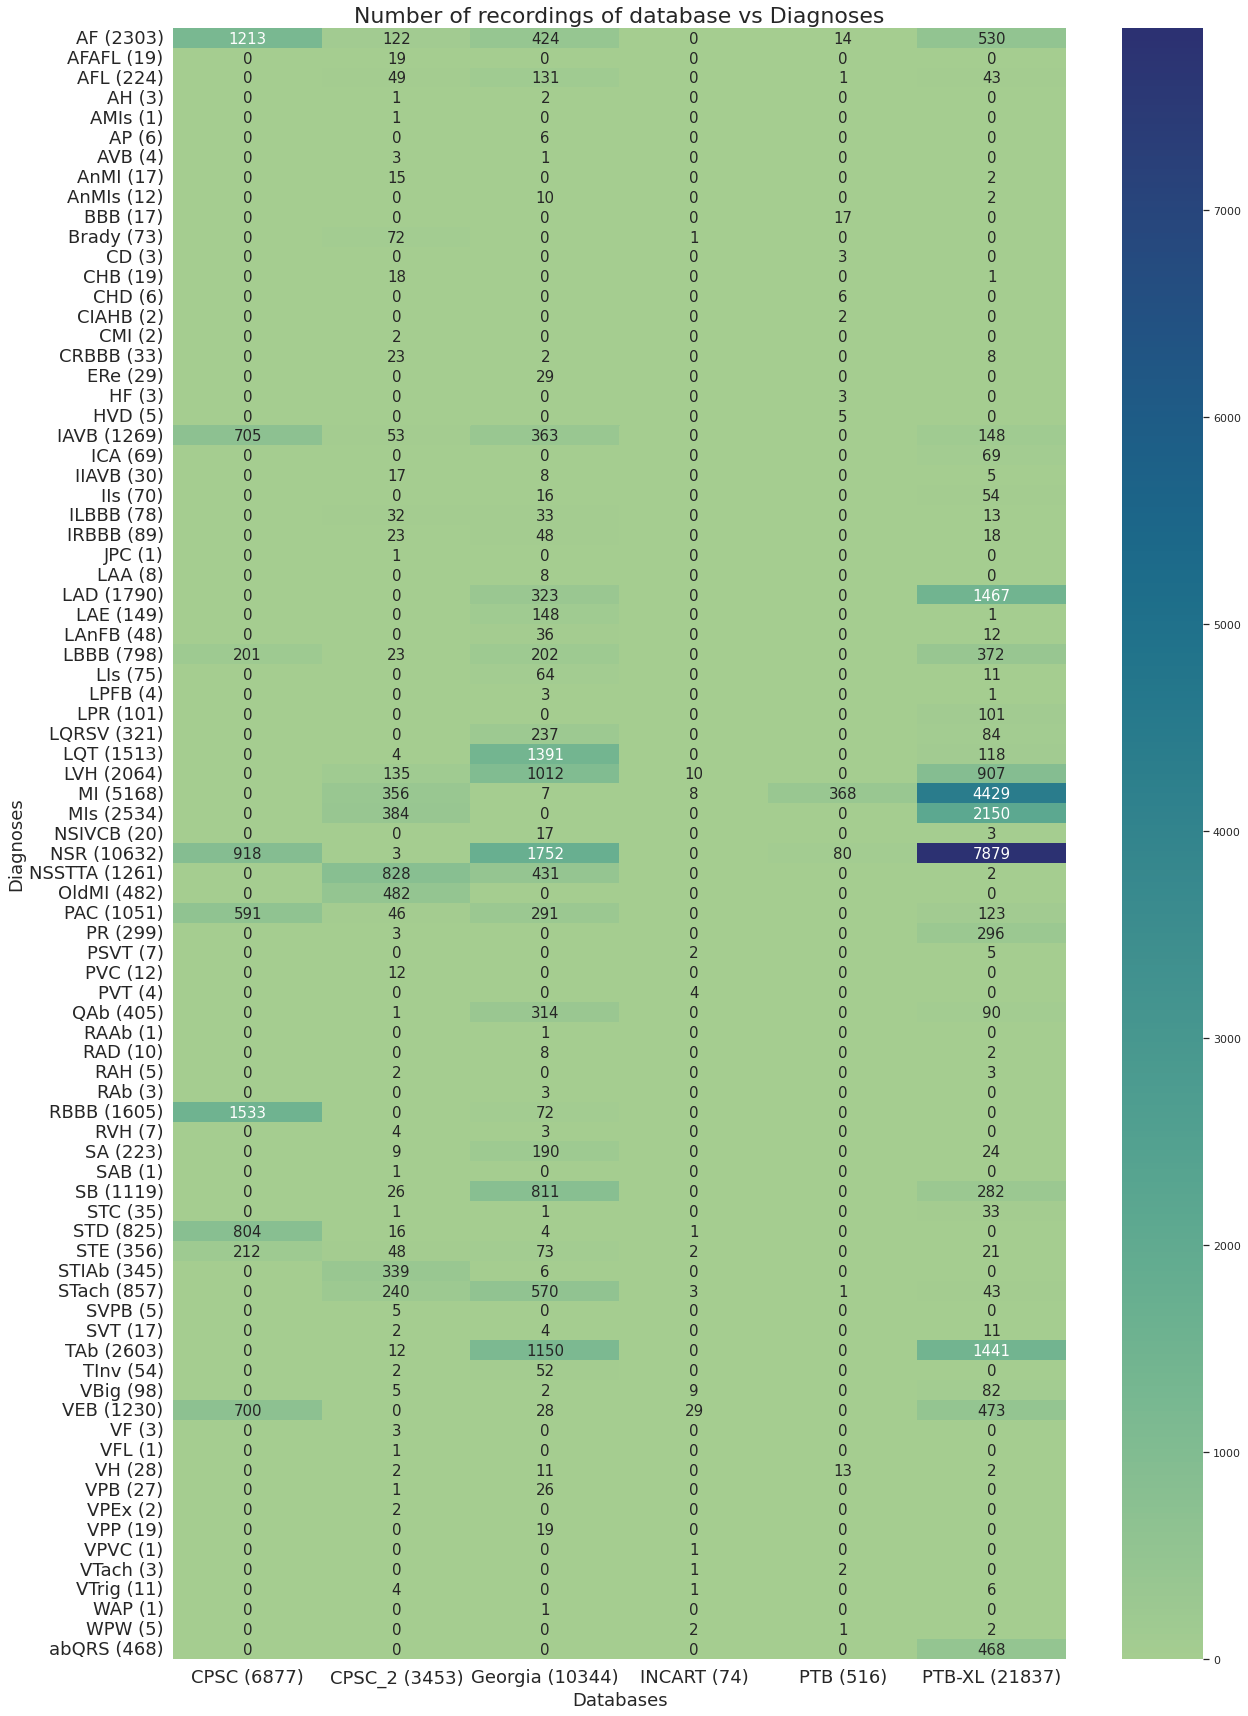
\includegraphics[scale=0.3]{img/diagnose_count_by_db.png}
\caption{Number of recordings for each diagnosis by database}
\label{fig:diagnose_count_by_db}
\end{figure}

All data is provided in WFDB format. Each ECG recording has a binary \textbf{MATLAB v4 file} for the ECG signal data and a \textbf{text file} in WFDB header format describing the recording and patient attributes, including the diagnosis \cite{dataset3} \cite{dataset2} \cite{dataset4}.

\section{Centralized Learning} \label{5CL}

To get an understanding of the best performances achievable with the mentioned dataset I implemented a Centralized (or traditional) Learning. The latter means that I applied the analytical tools mentioned in \ref{chap4} over the complete dataset, without dividing it into clients. Then the main processes and results are summarized in the following literals.

\subsection{Data wrangling}

As mentioned in \ref{4dw}, the data wrangling process is usually the first step when dealing with a data-oriented problem. In this case, I placed the data in a Google Drive folder after downloading it from the official competition's website \cite{dataset3}. Afterwords, using Google Colaboratory I extracted and organized the information in Python. The representation of the ECG along the 12-leads can be examined in Figure \ref{fig:ecg_example_S0033}.

\begin{figure}[H]
\centering
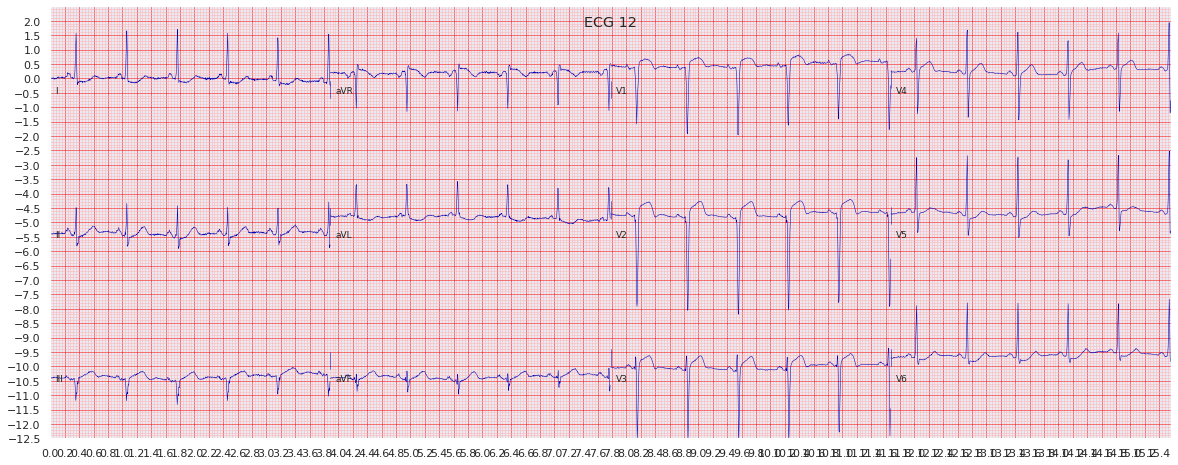
\includegraphics[scale=0.35]{img/ecg_example_S0033.png}
\caption{12-lead ECG for recording S0033 of PTB database}
\label{fig:ecg_example_S0033}
\end{figure}

Then, the whole data (all the databases) and the features mentioned in \ref{4fe} were calculated. That process took almost 1 hour to run in an using the default configuration of Google Colab. Besides, for each recording I selected the first diagnose (arrhythmia) that appeared as the label to be predicted. The latter process ran in about 2 minutes.

\subsection{EDA}

Once the big dataset was loaded, it contained a total of 43,101 recordings and about 764 variables. From the latter, 650 features got created containing 14 competition provided features and 636 were spectral features. There were remaining 3 corresponded to the id of the recording, the database that it belongs to and the label (response variable to be predicted). Then, the first analysis need was to examine if the features contained any missing value. Using the function \texttt{bar} from the \texttt{missingno} library, I managed to explore the missing values. In figure \ref{fig:eda_missing} are depicted only the 50 first features' missing counts and percentage.

\begin{figure}[H]
\centering
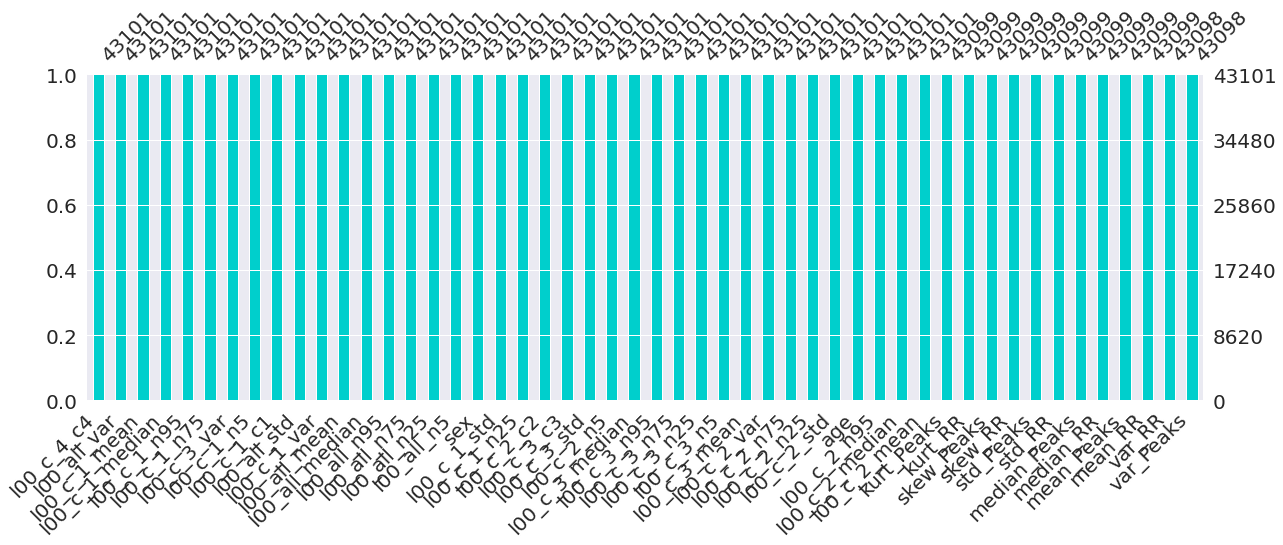
\includegraphics[scale=0.32]{img/eda_missing.png}
\caption{Missing counts and percentage for 50 features of the complete dataset}
\label{fig:eda_missing}
\end{figure}

As shown in the previous chart, the missing percentage is considerably small (less than 0.1\%). For that reason, I decided to impute those missing values by using the mean (average) of each attribute. 

The second crucial aspect to investigate was the distribution of the response variable. Then, within the plot \ref{fig:label_ditro_alldata} it is shown the absolute count of each diagnose in the dataset.

\begin{figure}[H]
\centering
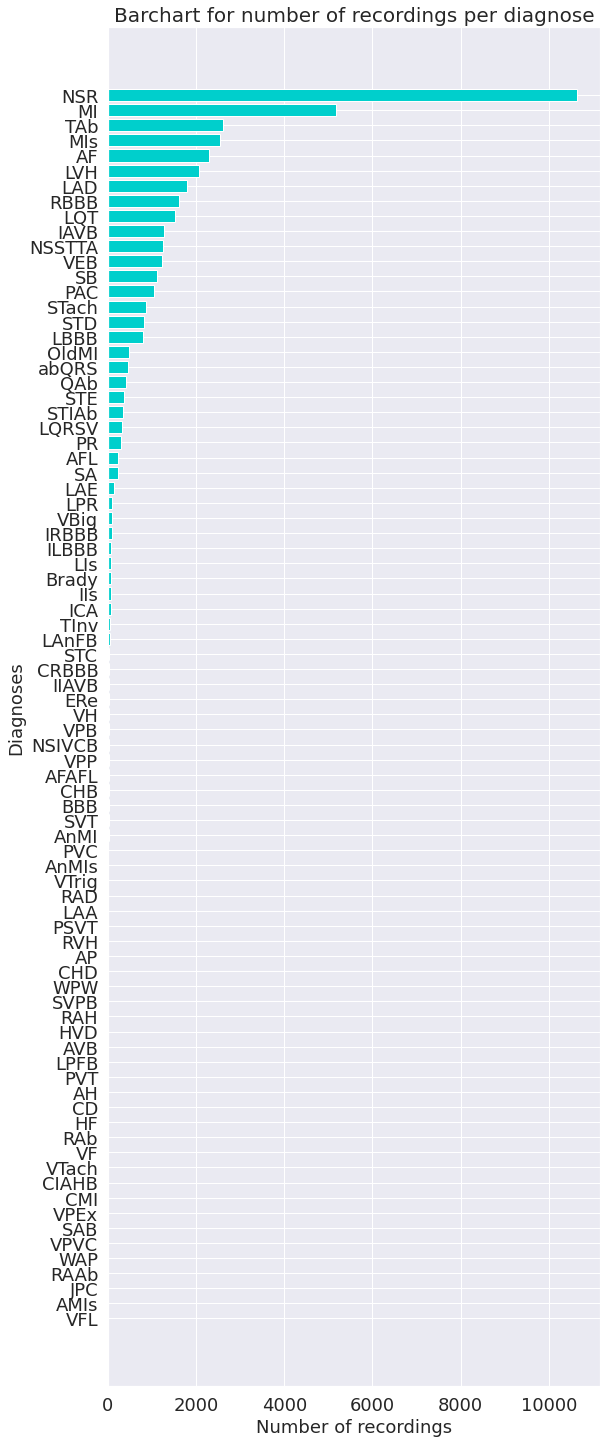
\includegraphics[scale=0.32]{img/label_ditro_alldata.png}
\caption{Label distribution for the complete dataset}
\label{fig:label_ditro_alldata}
\end{figure}

As evidenced in the previous chart, there are too many arrhythmias that don't have a big participation. That can lead to problems when trying to infer the predicted class of a recording, since there were not enough cases to learn the classifiers properly. That why those diagnoses with a participation smaller than 150 records where discarded from the analysis. With the previous filter, the selected data to work with got a size of 41,894 recordings distributed as shown in figure \ref{fig:diagnose_count_by_db_filtered}.

\begin{figure}[H]
\centering
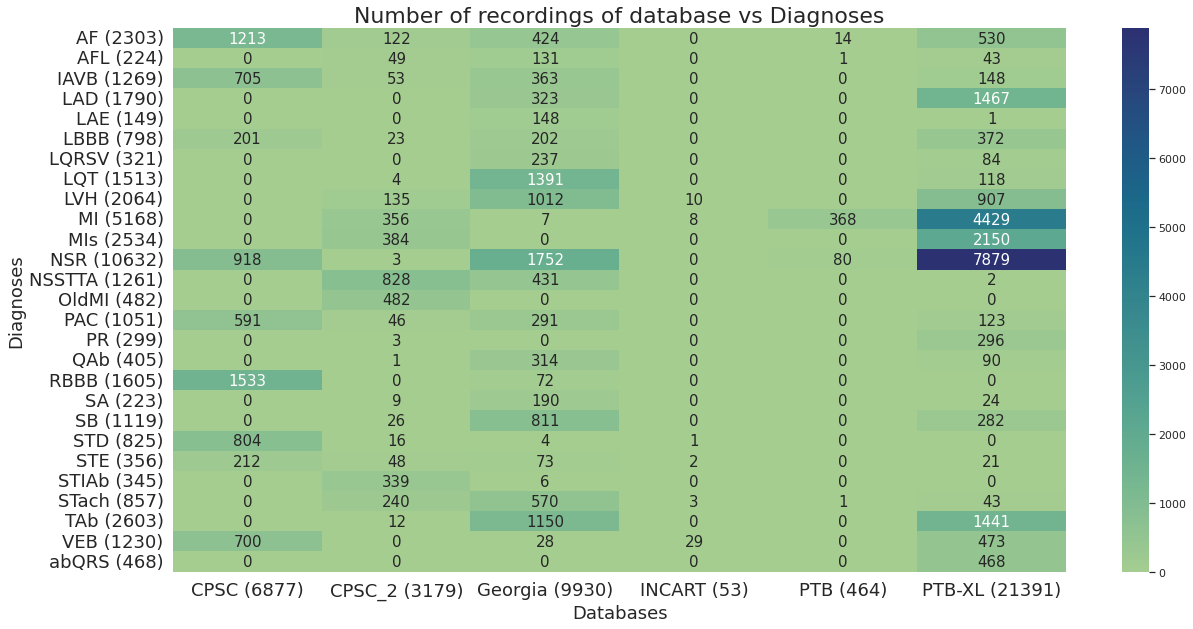
\includegraphics[scale=0.32]{img/diagnose_count_by_db_filtered.png}
\caption{Number of recordings for each diagnosis by database for the filtered data}
\label{fig:diagnose_count_by_db_filtered}
\end{figure}

Besides, the final distribution of the labels ended up as shown in figure \ref{fig:label_ditro_filtered}. As expected, the most common diagnose was Normal Sinus Rhythm (NSR), which is the normal status for a ECG. In addition. the arrhythmia with one of the smallest participation turned out to be Sinus Arrhythmia (SA).

\begin{figure}[H]
\centering
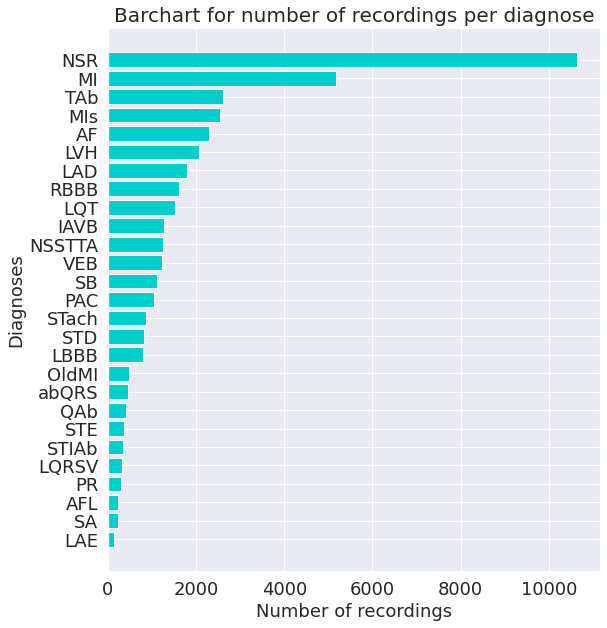
\includegraphics[scale=0.32]{img/label_ditro_filtered.png}
\caption{Label distribution for the filtered dataset}
\label{fig:label_ditro_filtered}
\end{figure}

\subsection{Feature Selection and normalization}

In an analytical context, having a huge amount is a double-edged sword. On the one hand, the more information existing to predict a phenomena, the better. On the other hand, the computational time required to process to much information may lead to training times that are not affordable. Regarding the latter I decided to perform a feature selection step in order to determine the most important features to predict the arrhythmias. 

\begin{figure}[H]
\centering
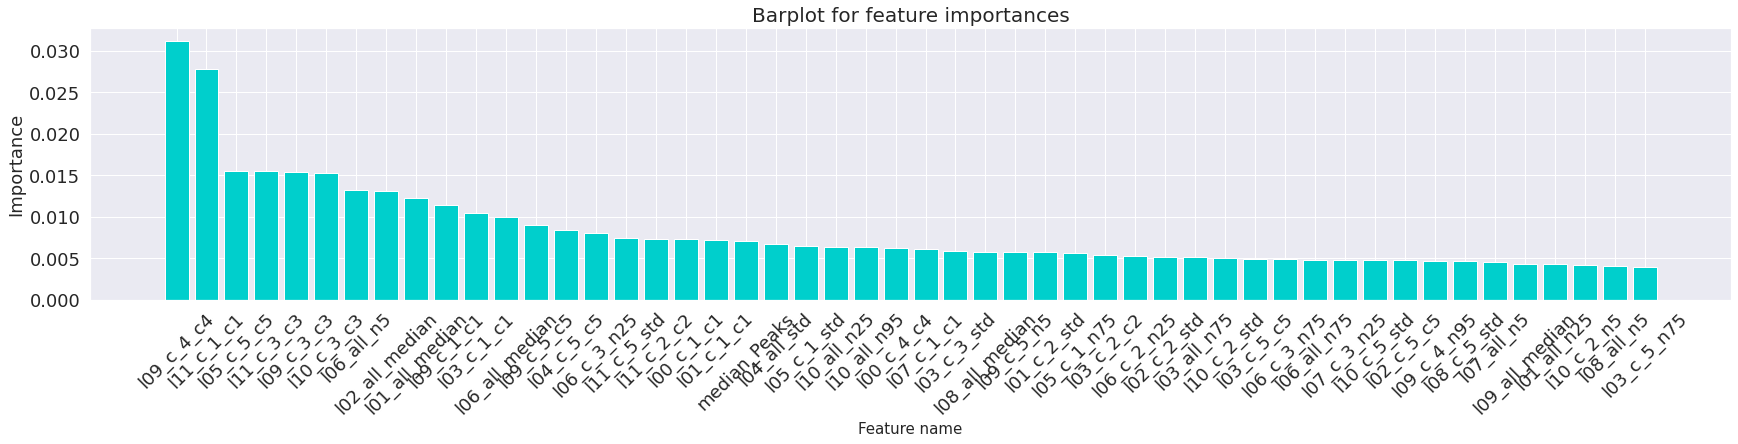
\includegraphics[scale=0.23]{img/feature_importance.png}
\caption{Feature importance from XG-Boost algorithm (only the 50 best)}
\label{fig:feature_importance}
\end{figure}

The bar-plot in figure \ref{fig:feature_importance} depicted the most important features to predict the classes obtained by means of the XG-Boost method. The latter provides an automatic ranking of the most relevant features to classifier the ECGs. After having importance of features of all 650 features, next step was to try to reduce the unimportant features and
run the model. During various trial run and keeping F1-Score as primary metric reducing ranked features from 150 -100 F1-score went down from 0.56 to 0.52 and keeping it on 120 features it goes back to 0.56. So, in the end, 120 features got selected which leads to good enough accuracy and f1-
score compared to the one obtained using all the features.The best features turned out to be the Entropy for leads: 9, 11, 10; the percentile 5\% for lead 6; and the median for leads 1, 2.

As an additional tool to enhance the performance of the models there was an implementation of features \textbf{normalization}. In this case I tried three different techniques to transform the features to the same scale. The approaches tried were provided by the \texttt{sklearn} library in Python. Those are: \texttt{StandardScaler}, \texttt{MaxMinScaler} and \texttt{RobustScaler}. In the end, the scenario that provided the best results was using \texttt{RobustScaler}. 

\begin{equation} \label{robustscaler_eq}
X_{scale} = \frac{x_i - x_{med}}{x_{75} - x_{25}}
\end{equation}

\texttt{RobustScaler} [\ref{robustscaler_eq}] uses statistics that was resistant to outliers to scale features. The median removed, and the data scaled according to the quantile range (defaults to IQR: Interquartile Range). The interquartile range (IQR) is the distance between the first and third quartiles (25th and 3rd quantiles) (75th quantile). It is worth mentioning that centering and scaling happen independently on each feature by computing the relevant statistics on the samples in the given dataset.

\subsection{Balancing classes (arrhythmias)}

As depicted in \ref{fig:label_ditro_filtered}, the diagnoses have a imbalanced characteristic. The latter means that each category has a different participation over the data. That could represent a problem in the performance of the classifiers that will be proposed.

\begin{figure}[H]
\centering
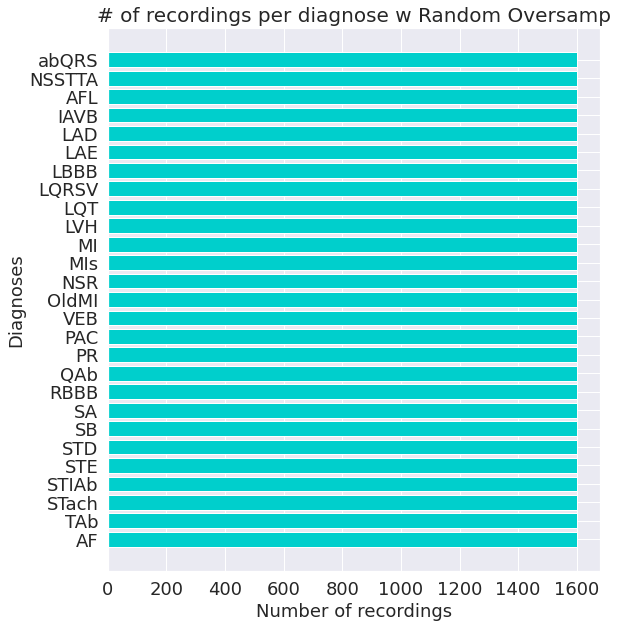
\includegraphics[scale=0.4]{img/label_distro_ros.png}
\caption{Number of recordings for each diagnosis by database for the ROS oversampled data}
\label{fig:label_distro_ros}
\end{figure}

Then, two oversampling methods were proposed to deal with the imbalance issue. The first one is called \textbf{Random Oversampling (ROS)}. In the latter the minority classes are replicated together with its features. Besides, a down-sampling was applied to have a number of recording similar to the filtered dataset. In the end, the ROS dataset had 43,200 recordings. And as depicted in figure \ref{fig:label_distro_ros}, the distribution of the labels is much more similar among the arrhythmia categories.

\begin{figure}[H]
\centering
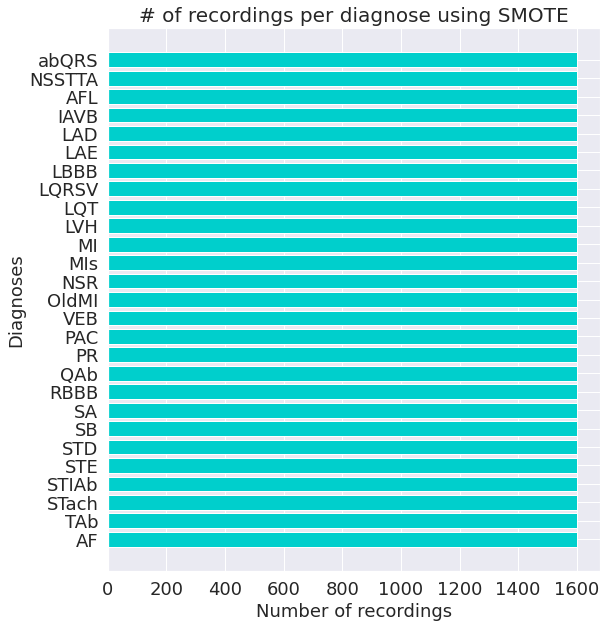
\includegraphics[scale=0.4]{img/label_distro_smote.png}
\caption{Number of recordings for each diagnosis by database for the SMOTE oversampled data}
\label{fig:label_distro_smote}
\end{figure}

The second oversampling technique used was SMOTE (SMT) \ref{3unbclass}. In the end, the SMOTE dataset had also 43,200 recordings. And as shown in figure \ref{fig:label_distro_smote}, the distribution of the labels is also similar among the arrhythmia categories.

\subsection{Fitted models and results}

With the previous pre-processing applied over the data, the following step was to adjust some Machine Learning models to the ECG's arrhythmias. During this step also other scenarios and considerations were employed \cite{datasplit}. A detailed explanation of the outlines is discussed in table \ref{table:scenarios_models}.

\begin{table}[H]
\begin{center}
\begin{tabular}{ ||p{3cm}||p{5cm}||p{4cm}|| }
 \hline
\textbf{Characteristic} & \textbf{Scenarios} & \textbf{Best approach}\\ [0.4ex] 
 \hline\hline
 Data Split & \%Train-\%Validation-\%Test: Option 1: 60\%-20\%-20\% Option 2: 70\%-10\%-10\% Option 3: 80\%-10\%-10\% Option 4: 90\%-5\%-5\% & Option 4: 90\%-5\%-5\%\\
\hline
Features normalization & Option 1: MinMaxScaler \hspace{10 mm} Option 2: StandardScaler \hspace{10 mm} Option 3: RobustScaler & Option 3: RobustScaler \\
\hline
Sampling rate & Option 1: 257Hz \hspace{10 mm} Option 2: 500Hz & Option 1: 257Hz \\
\hline
Features employed & Option 1: Baseline features Option 2: Baseline features + Spectral features & Option 2: Baseline features + Spectral features \\
\hline\hline
\end{tabular}
\end{center}
\caption{Scenarios tried during modelling phase}
\label{table:scenarios_models}
\end{table}

In the previous table are depicted the best approaches that managed to get the best performances (in terms of Accuracy, Recall, Precision, F1-Score and Overall Score). Moreover, in figure \ref{fig:cl_oindex_methods} is shown the detailed behaviour of each one of the algorithms employed.

\begin{figure}[H]
\centering
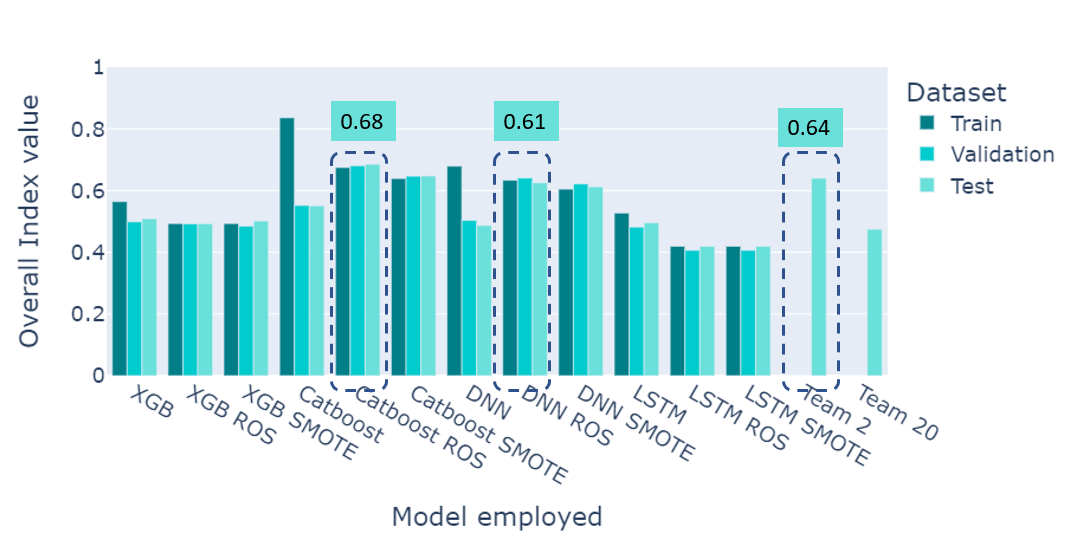
\includegraphics[scale=0.5]{img/cl_oindex_methods.png}
\caption{Overall Index for methods employed in Centralized Learning (CL)}
\label{fig:cl_oindex_methods}
\end{figure}

Within the previous results it is easy to realize that the champion model is the one that applies Catboost over the ROS data. The latter obtained an overall index close to 0.68. Competition team which ranked 2 is at the second position having overall index as 0.64. This model was trained over above \ref{table:scenarios_models} scenario having trained data as 90\%, 5\% validation data and 5\% for testing and same pattern has been followed on team 20 analysis. Nevertheless, the Deep Neural Network (DNN) applied over the ROS data has a close behaviour, having a the mentioned metric in 0.61. Finally, LSTM and XG-Boost does not perform that well compared to the other models. An additional point to mention is that both Catboost and DNN used over the ROS dataset does not show any sign of overfitting since the metrics for train, validation and test sets are almost the same. As for team 2 and team 20 in the above figure train and validation overall index is not shown because they followed their own pattern keeping in mind the competition score during training and validation. 

\begin{figure}[H]
\centering
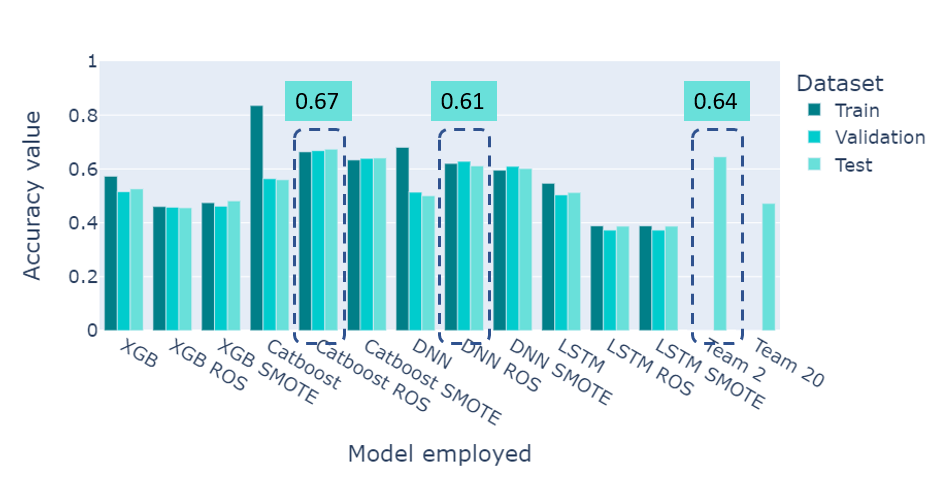
\includegraphics[scale=0.55]{img/cl_accuracy_methods.png}
\caption{Accuracy for methods employed in Centralized Learning (CL)}
\label{fig:cl_accuracy_methods}
\end{figure}

\begin{figure}[H]
\centering
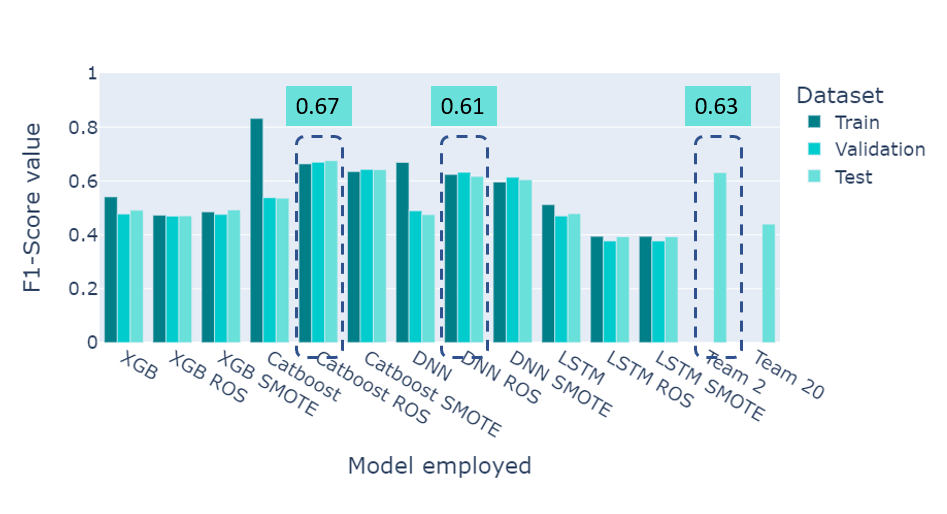
\includegraphics[scale=0.55]{img/cl_f1score_methods.png}
\caption{F1-Score for methods employed in Centralized Learning (CL)}
\label{fig:cl_f1score_methods}
\end{figure}

A similar analysis can be derived from figures \ref{fig:cl_accuracy_methods} and \ref{fig:cl_f1score_methods}, where the Accuracy and F1-Score are shown. In terms of Accuracy, Catboost got 0.67, team 2 got 0.64 and DNN got 0.61 while applied over the ROS dataset. It is important to clarify that using Accuracy is not a the best metrics in this dataset since the labels are heavily unbalanced. For that reason, it is better to use the F1-Score. which is more robust to the imbalanced datasets. Then, in terms of F1-Score, Catboost obtained a 0.67, team 2 model got 0.63 and DNN 0.62.

\begin{figure}[H]
\centering
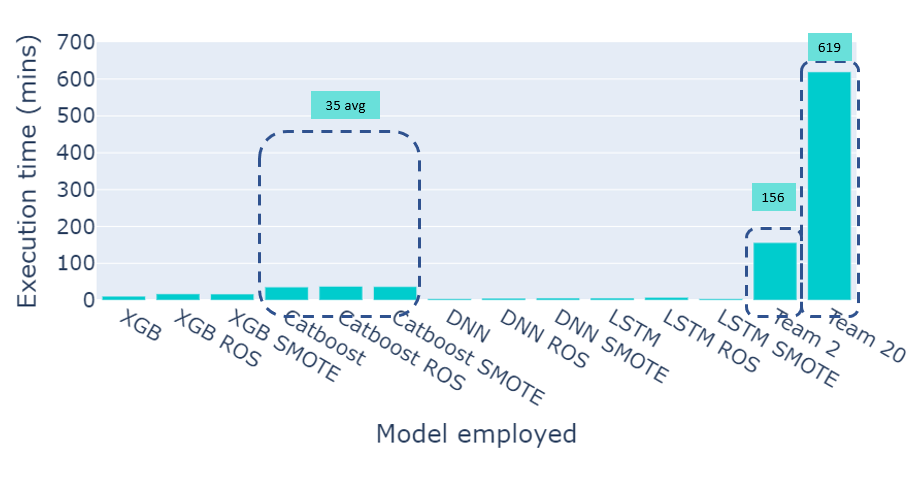
\includegraphics[scale=0.6]{img/time_cl_teams.png}
\caption{Execution times for the methods used in CL}
\label{fig:times_cl}
\end{figure}

Finally, a measurement of the time taken to train for each model was included. As shown in figure \ref{fig:times_cl}, Team 20 model took almost 619 minutes, team 2 took 156 minutes and Catboost took almost 35 minutes to run. On the other hand, DNN and LSTM are algorithms that employed a few time in training (close to 4 minutes in average). Finally, Catboost is the slowest method, although it generates the best results. In counter position, DNN is the fastest method, and the performance is NOT quite different from Catboost and team 2 model. Team 2 and team 20 models took this much time because they are end to end models instead of feature based model. Although I have done some experiments on team 2 which will be explained below. 


\section{Conversion to Tensorflow Lite } \label{5CTL}

 We can convert potentially any model that is built using TensorFlow core libraries and tools. Once you've built a model with TensorFlow core, you can convert it to a smaller, more efficient ML model format called a TensorFlow Lite. Also, there are other advanced steps related to it if your model is built using tensorflow core libraries by looking at the steps here  \ref{fig:model_conversion_process} we can convert models that are built using either in Pytorch or Matlab. 
 
 
\subsection{Model 1(XGBoost) and Model 2(Catboost) conversion}\label{5CTLM1M2}

As both of \href{https://xgboost.readthedocs.io}{XGBoost} and \href{https://catboost.ai}{Catboost} are not built using Tensorflow even there is no direct conversion available I opted out to use trained models built on top of CatBoost and XGBoost. Just to keep in mind that both of these libraries somehow support directly or indirectly iOS platform but not the android. As after conversion I am going to use directly in both iOS/Android to see how they perform in real world scenarios. 

\subsection{Model 3(LSTM)}\label{5CTLM3}

LSTM model is built on top of Tensorflow so it was convertable to tensorflow lite. If we look at LSTM models of simple LSTM, LSTM ROS, LSTM SMOTE, better F1-score and overall index is achieved by simple LSTM model with 0.49 overall index and 0.47 F1-score. LSTM had one problem during conversion step it had two sub graphs which is not supported by tensorflow lite models. To overcome this problem \textbf{TFLite LSTM op } was used and at the end we get the graph that had only one subgraph.


\begin{figure}[H]
\centering
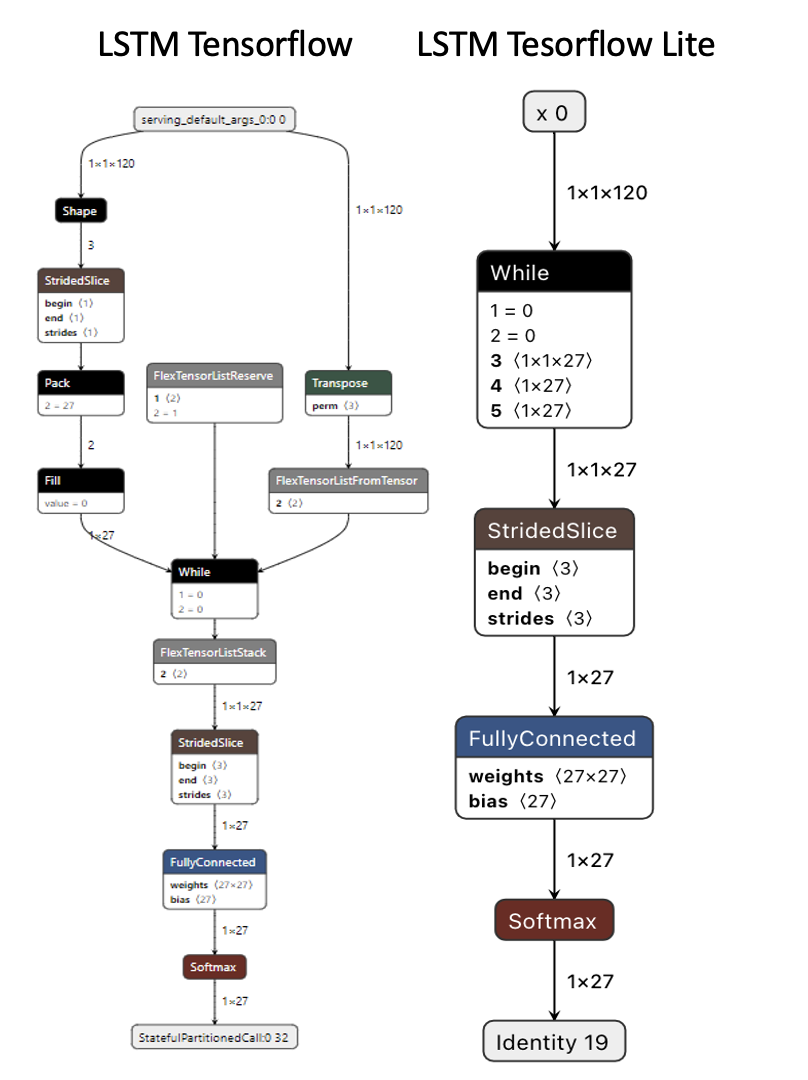
\includegraphics[scale=0.7]{img/lstm_conversion_comparison.png}
\caption{Tensorflow LSTM model's graph to Tensorflow Lite model's graph comparison}
\label{fig:lstm_conversion_comparison}
\end{figure}


As you can see in \ref{fig:lstm_conversion_comparison}, LSTM Tensorflow original model and Tensorlow Lite model after conversion step taken place using TFLite LSTM op. 

\subsection{Model 4(DNN)}\label{5CTLM4}

As DNN model was also built using Tensorflow with 4 fully connected layers 3 with 500 neurons output in each and relu as activation function with output. In the fourth layer, it has to output 27 classes of arythmia's with probabilities so it using Softmax in the last layer. To look at its graph in tensorflow lite model it is not that interesting and the only intresting thing to note that tensorflow lite as I have converted only support one input at a time and Tensorflow one can support batches of inputs as well. As, I have to use Tensoflow lite version in mobile so most probably it will be given an input to classify one at a time. 


\begin{figure}[H]
\centering
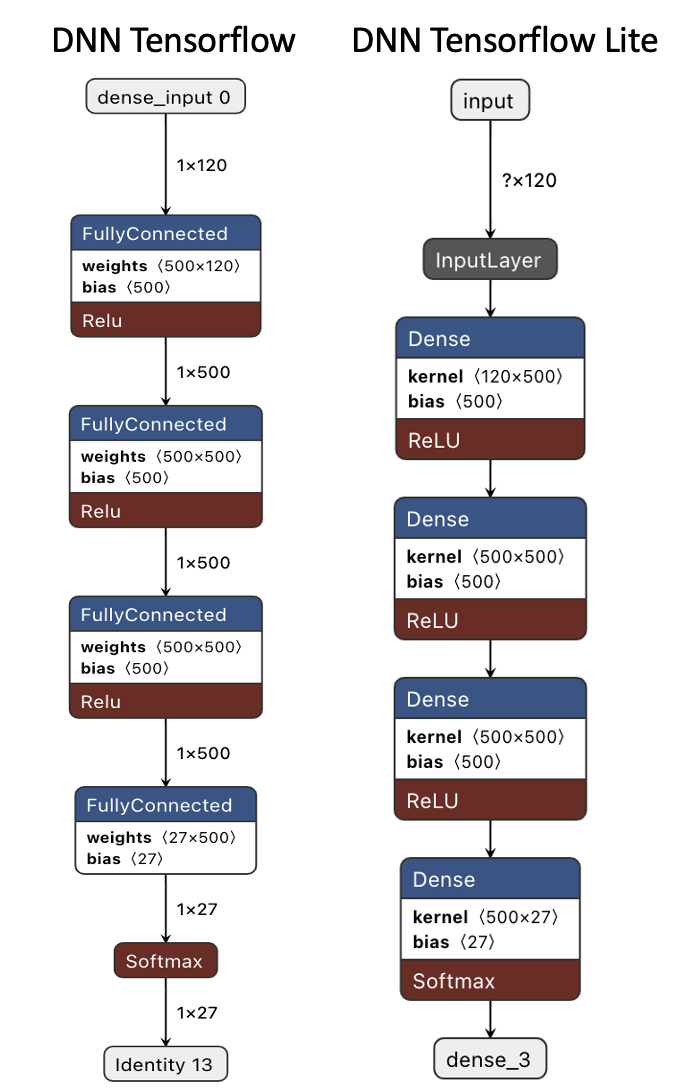
\includegraphics[scale=0.7]{img/dnn_conversion_comparison.png}
\caption{Tensorflow DNN model's graph to Tensorflow Lite model's graph comparison}
\label{dnn_conversion_comparison}
\end{figure}


\subsection{Model 5 - Challenge Team 2}\label{5CTLM5}

As challenge 2 team was using Pytorch instead of Tensorflow as primary framework library to build the model. I have to convert the model following all the steps mentioned in \ref{fig:model_conversion_process}. So, first trained model .pt file is converted to ONNX format and get tested, then it got converted to .pb file and at the end when .pb get imported to tensorflow it got directly converted to Tensorflow lite. As challenge team 2 was using ensemble approach where they were using 5 models which got trained over shuffled dataset for training and validation. We will look at the first model in .pt format how it looks and then converted model in Tensorflow Lite as comaprison. Also, this model length is too big to compare it here I will be using first few layers as comparison here. 

\begin{figure}[H]
\centering
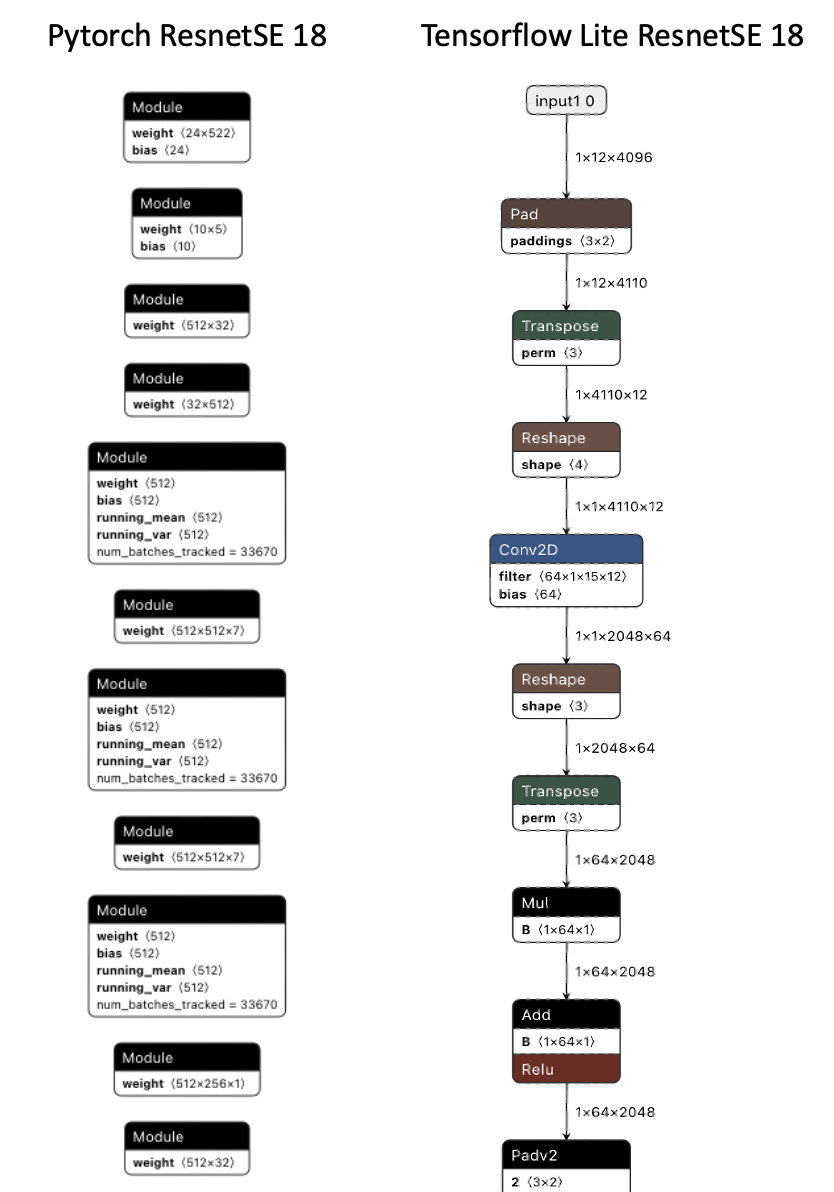
\includegraphics[scale=0.7]{img/resnetse_conversion_comparison.png}
\caption{Pytorch ResnetSE 18 model's graph to Tensorflow Lite model's graph comparison }
\label{resenet18_conversion_comparison}
\end{figure}

As we can see in \ref{resenet18_conversion_comparison} during conversion to tensorflow lite there are too many operation that gets performed including pad, Transpose, Reshape, Mul and etc. So, we can conclude that in conversion process to Tensorflow Lite there are additional operations gets added to model graphs to support some of complex operations. 


\subsection{Model 6 - Challenge Team 20}\label{5CTLM6}

As Challenge team 20, worked directly on Tensorflow framework library it was easy to convert the model to Tensorflow Lite directly. Lets look at the original model and converted model comparison side by side. It is also important to mentioned that as they were training 10 different models using shuffled dataset and I choose the one for comaprison which were performing better in Accuracy, F1 measure and overall index. It is important to note that difference between these models was really small it terms of metrics as mentioned before. Model graph length is too big to paste it here so I will be comparing first few layers of it as in the case of Model 5. \ref{5CTLM5} 


\begin{figure}[H]
\centering
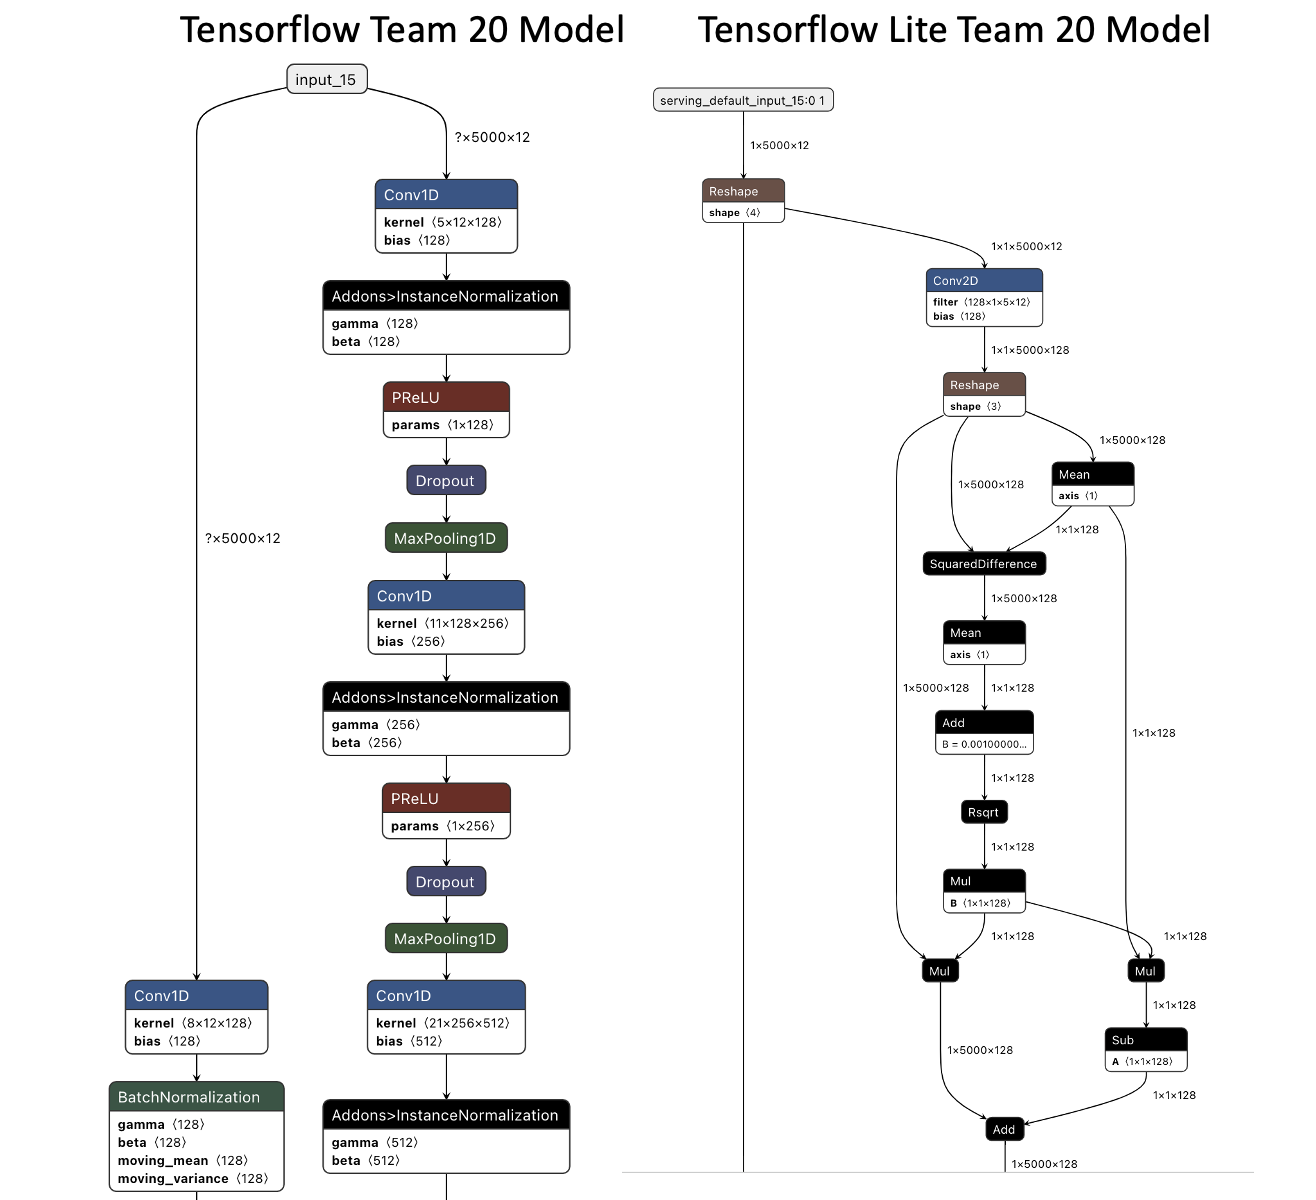
\includegraphics[scale=0.7]{img/team20_conversion_comparison.png}
\caption{Tensorflow Team 20 model's graph to Tensorflow Lite model's graph comparison}
\label{team20_conversion_comparison}
\end{figure}

Looking at above figure \ref{team20_conversion_comparison}, we can clearly see that in tensorflow lite graph there are multiple other operations that we haven't seen befofe like Sub, SquaredDifference, Mean, Rsqrt etc. It is evident all the complex operations get converted to more simpler operations in tensorflow lite format of the model.  



\subsection{Metrics of models}

As written previously, Catboost and XGBoost \ref{5CTLM1M2} are not convertible directly to tensorflow lite. Besides that other models were convertible and it was only worth to look at the models that performed well in terms of accuracy, f1-score and overall index because they will be later used for detecting arythmias in mobile applications. So, DNN ROS with overeall index as 0.62, LSTM with overall index as 0.49, Team 2 model with overall index as 0.64 and Team 20 model(CNN+Rule Based) with overall index of 0.47 was chosen for below analysis. 


\begin{figure}[H]
\subfloat[DNN ROS]{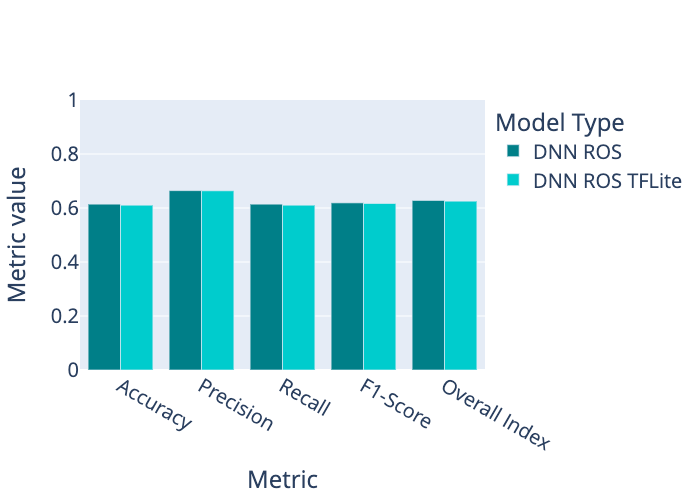
\includegraphics[width = 3in]{img/dnnros_metrics.png}} 
\subfloat[LSTM]{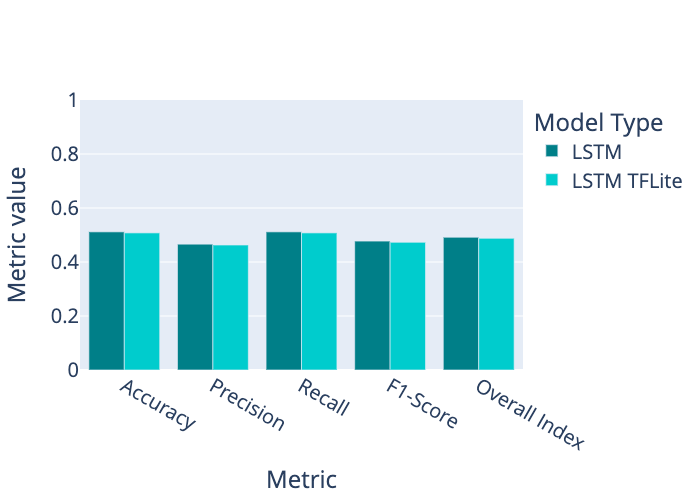
\includegraphics[width = 3in]{img/lstm_metrics.png}}\\
\subfloat[Team 2]{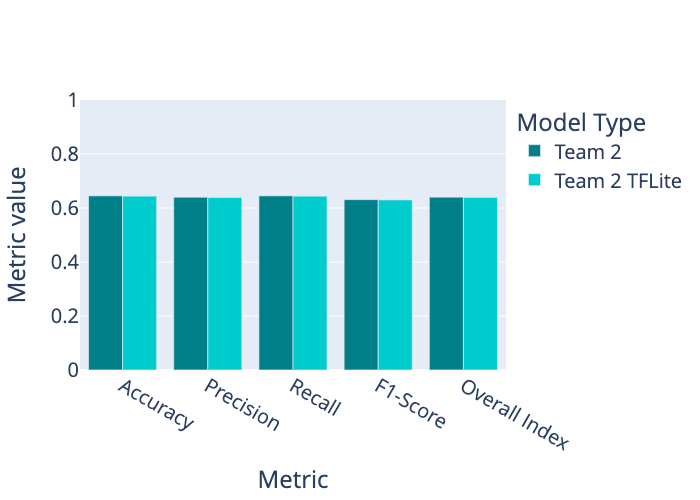
\includegraphics[width = 3in]{img/team2_metrics.png}}
\subfloat[Team 20]{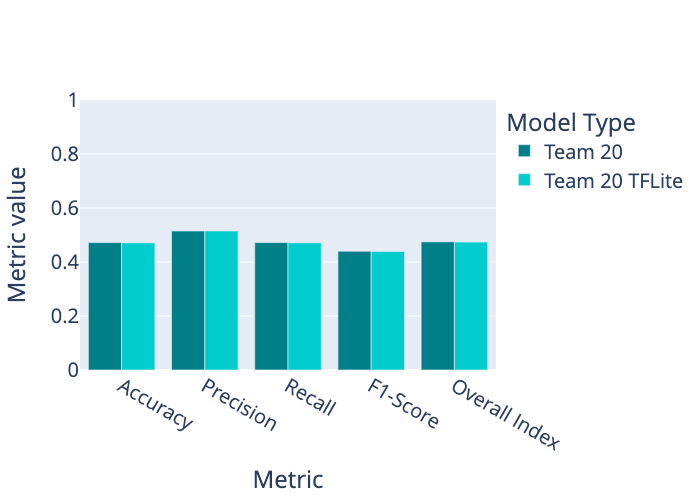
\includegraphics[width = 3in]{img/team20_metrics.png}} 
\caption{Metrics of models comparing side by side with original model and TF Lite version of the model}
\label{metricsafterconversion}
\end{figure}

If we look at above figures we can clearly see that a little drop in every metric after the model is converted to tensorflow lite. As, I didn't wanted the models to be quantize more so that their accuracy, f1-score decreases so I opted for tensorflow lite default conversion operations. 


Now if we move toward looking at how much time it takes the to get output from the model either before converting and after converting. There is huge difference when model is converted and we wanted to get the output from the model. It takes slighly and in case of hafty model it takes a lot more time. In real world scenario as we will not be using batching, or multiple inputs to get the output from the model because of that all above converted models only accept one input at a time. 

\begin{figure}[H]
\centering
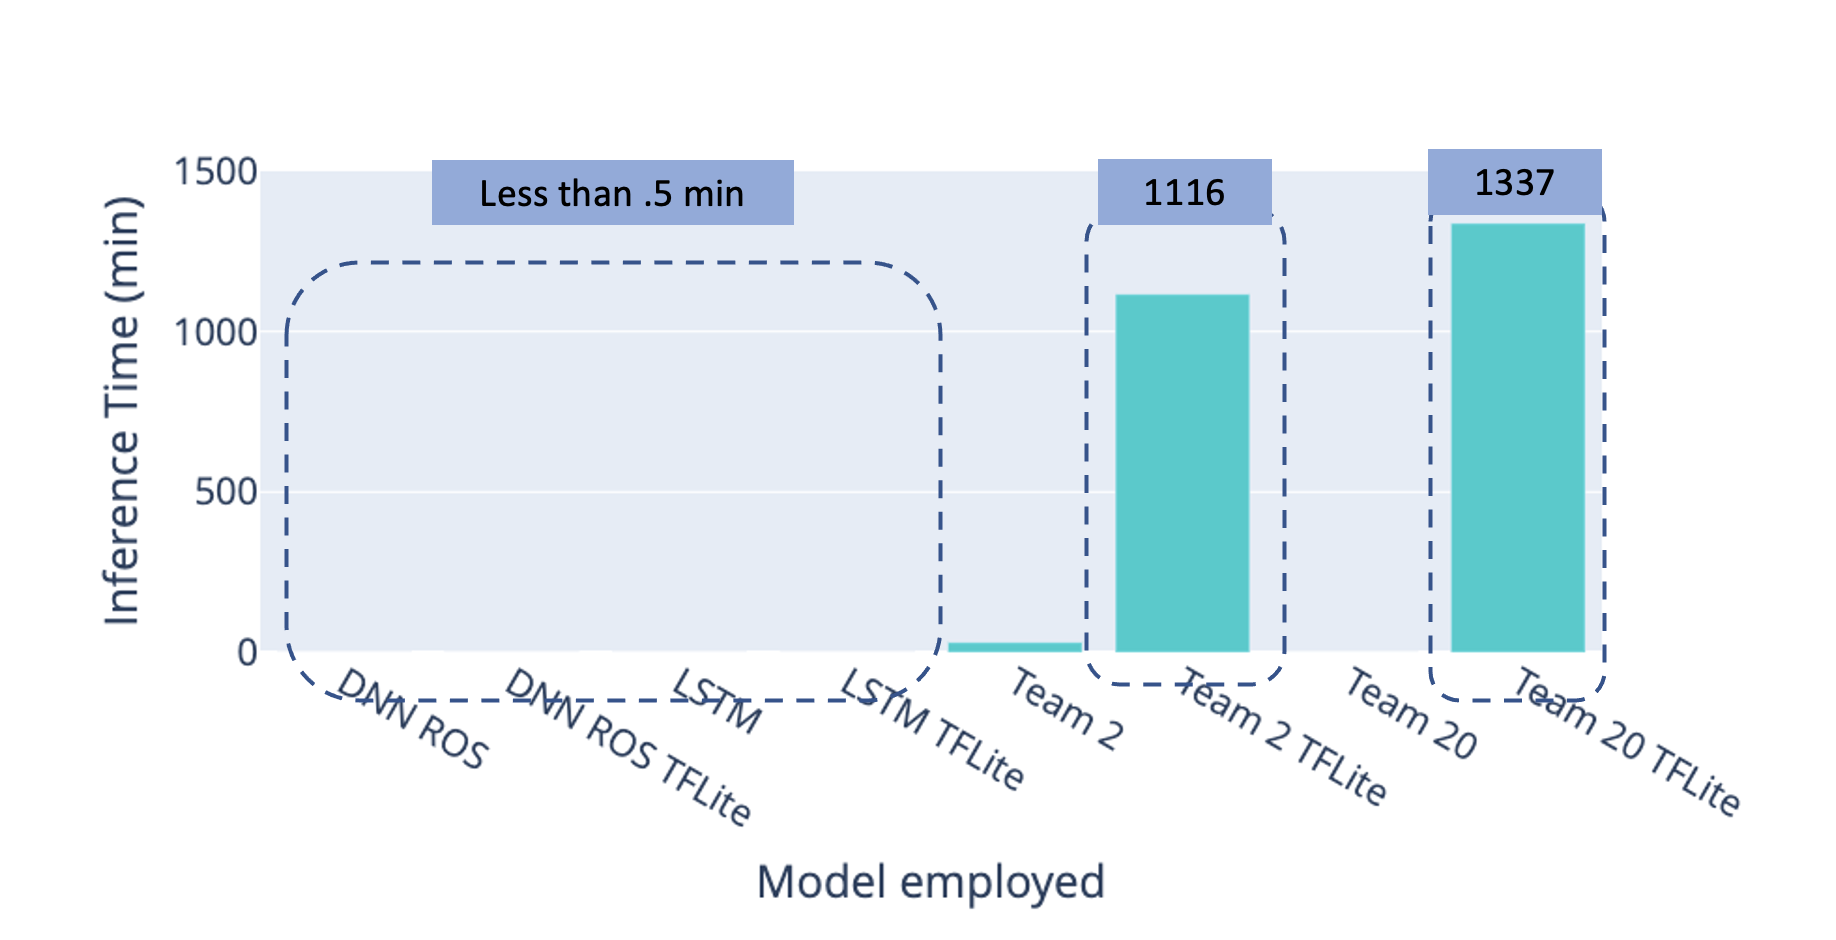
\includegraphics[scale=0.45]{img/inference_time_of_converted_models.png}
\caption{Inference Time in minutes of original and converted models}
\label{inference_time_of_converted_models}
\end{figure}

If we look at above \ref{figure:inference_time_of_converted_models} figure we can clearly see that LSTM and DNN ROS models are way faster than Team 2 and Team 2. LSTM and DNN ROS models even after conversion is taking less than 0.30 sec to execute. To put it more precisely orginal DNN on test dataset with 2095 features takes 19 seconds to get outputs and .13 seconds for inference in case of converted model which is even less than original model. If we look at LSTM it does the same 13 seconds for original model and 067 seconds on converted model. This means that somehow both DNN and LSTM has to perform less operations and gets lighter and efficient after conversion. While on the other hand Team 2 and Team 20 models takes significantly too much time to output the results. More precisely, in case of Team 2 model it takes 1826 seconds to output 2095 results and 66960 seconds in case of converted model which raises concerns because its significantly slower than original model. As in the case of team 20 inference on original model was significantly smaller as 9.4 seconds and inference on converted model was huge slower 80232 seconds. It maybe due to CPU or GPU inference, I didn't get a chance to look at it. 

\begin{table}
\centering
\begin{tabular}{ |p{5cm}||p{3cm}|p{3cm}|}
 \hline
 \multicolumn{3}{|c|}{Size of Models} \\
 \hline
 Model's Name& Original Size&Converted size\\
 \hline
 DNN ROS   & 2.2MB   &   569KB\\
 LSTM&  82KB   & \textbf{29KB} \\
 TEAM\#2 &33.8MB & 9.6MB\\
 TEAM\#20  & 138.8MB & 11.6MB\\
 \hline
\end{tabular}
 \caption{\label{tab:models_size_after_conversion}Comparison of model size from original to converted models}
 \end{table}
 
 As you can see from \ref{tab:models_size_after_conversion}, the smallest model is LSTM and it even gets smaller when converted to tensorflow lite. Team \#20 model is really huge and its get converted to 11.6MB. Maybe because of that it takes time during inference. 
 
\subsection{Models Deployment}

As part of the models testing on mobile devices after conversion. LSTM, DNN ROS and Team \#2 model has been deployed on the mobile devices while building a small demo application using flutter. \href{https://flutter.dev/}{Flutter} is an open-source UI software development kit created by Google. As flutter supports Tensorflow Lite models only Catboost, XGBoost are not deployed, as well as Team \#20 model because accuracy,f1-score of the team \#20 model is very less. 

In the demo application, two main packages has been used \href{https://pub.dev/packages/tflite\_flutter}{tflite\_flutter} and \href{https://pub.dev/packages/csv}{csv}. \textit{csv} package has been used to read csv files and \textit{tflite\_flutter} is used to inference converted models. 

\textbf{DNN ROS and LSTM}

For DNN ROS and LSTM, I saved the features of test dataset 5\% after normalizing and standardizing as explained above in csv file. This csv file is used directly for inputs to the models. Then as both models are trained to classify single arythmia. Output of the model is based on classifying 27 arythmia's so whichever arythmia type is at highest probability is shown as predicted and then two more types according to highest probabilities is shown in \ref{dnn_deloyment} 


\begin{figure}[H]
\centering
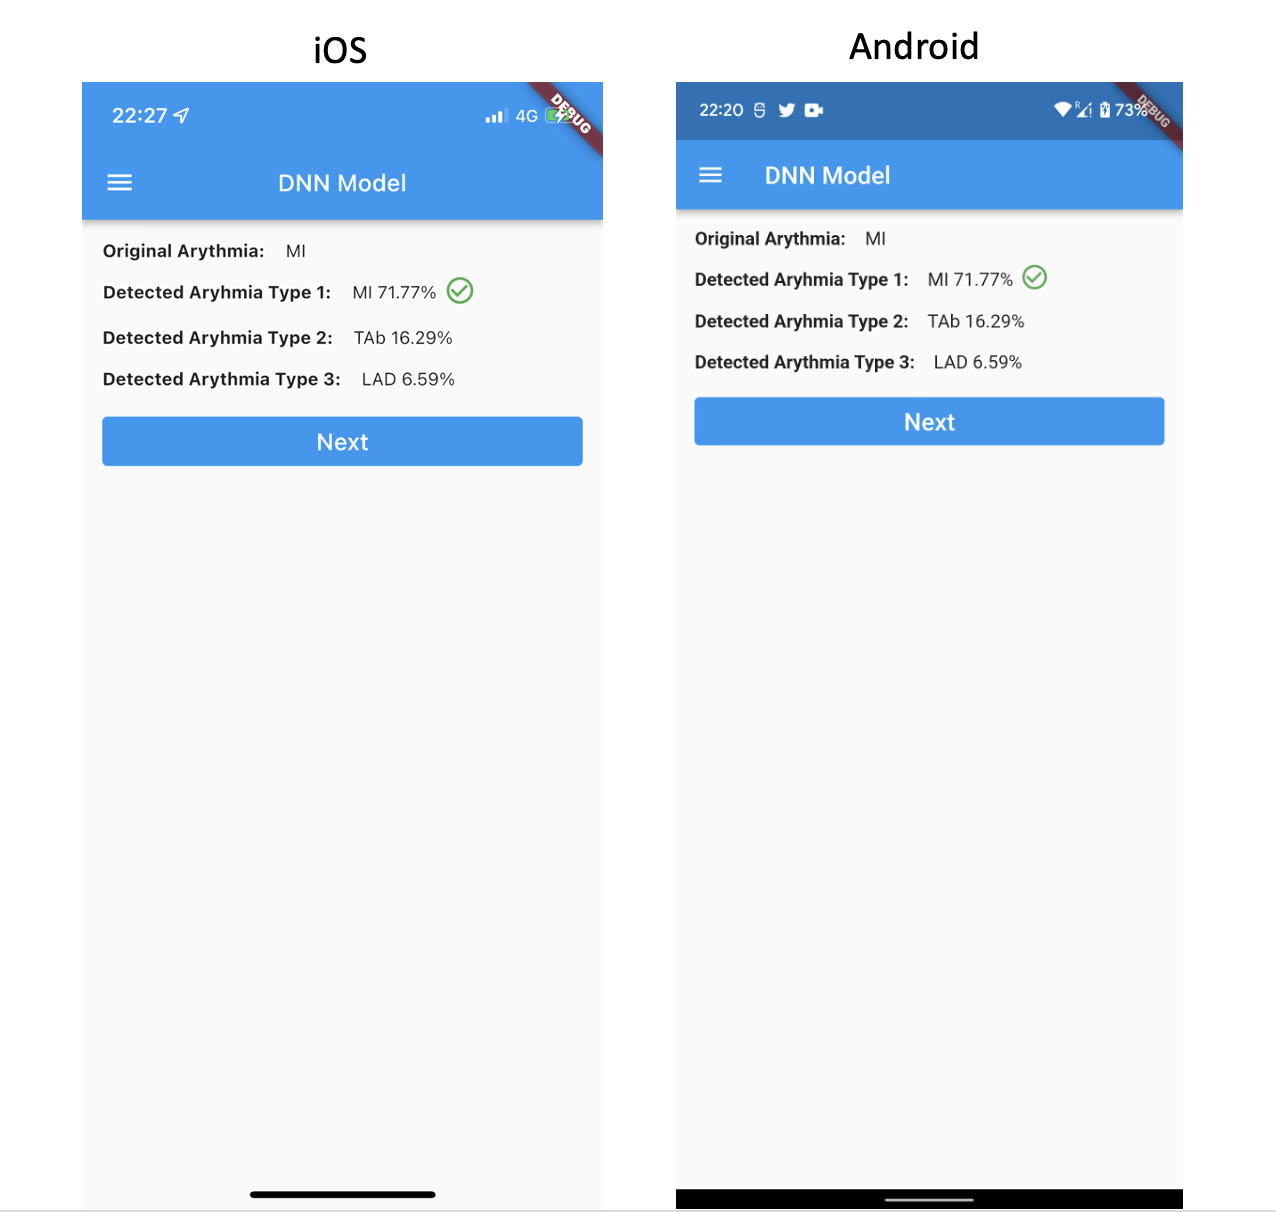
\includegraphics[scale=0.4]{img/dnn_deloyment.png}
\caption{iOS and Android DNN model classification example}
\label{dnn_deloyment}
\end{figure}

\begin{figure}[H]
\centering
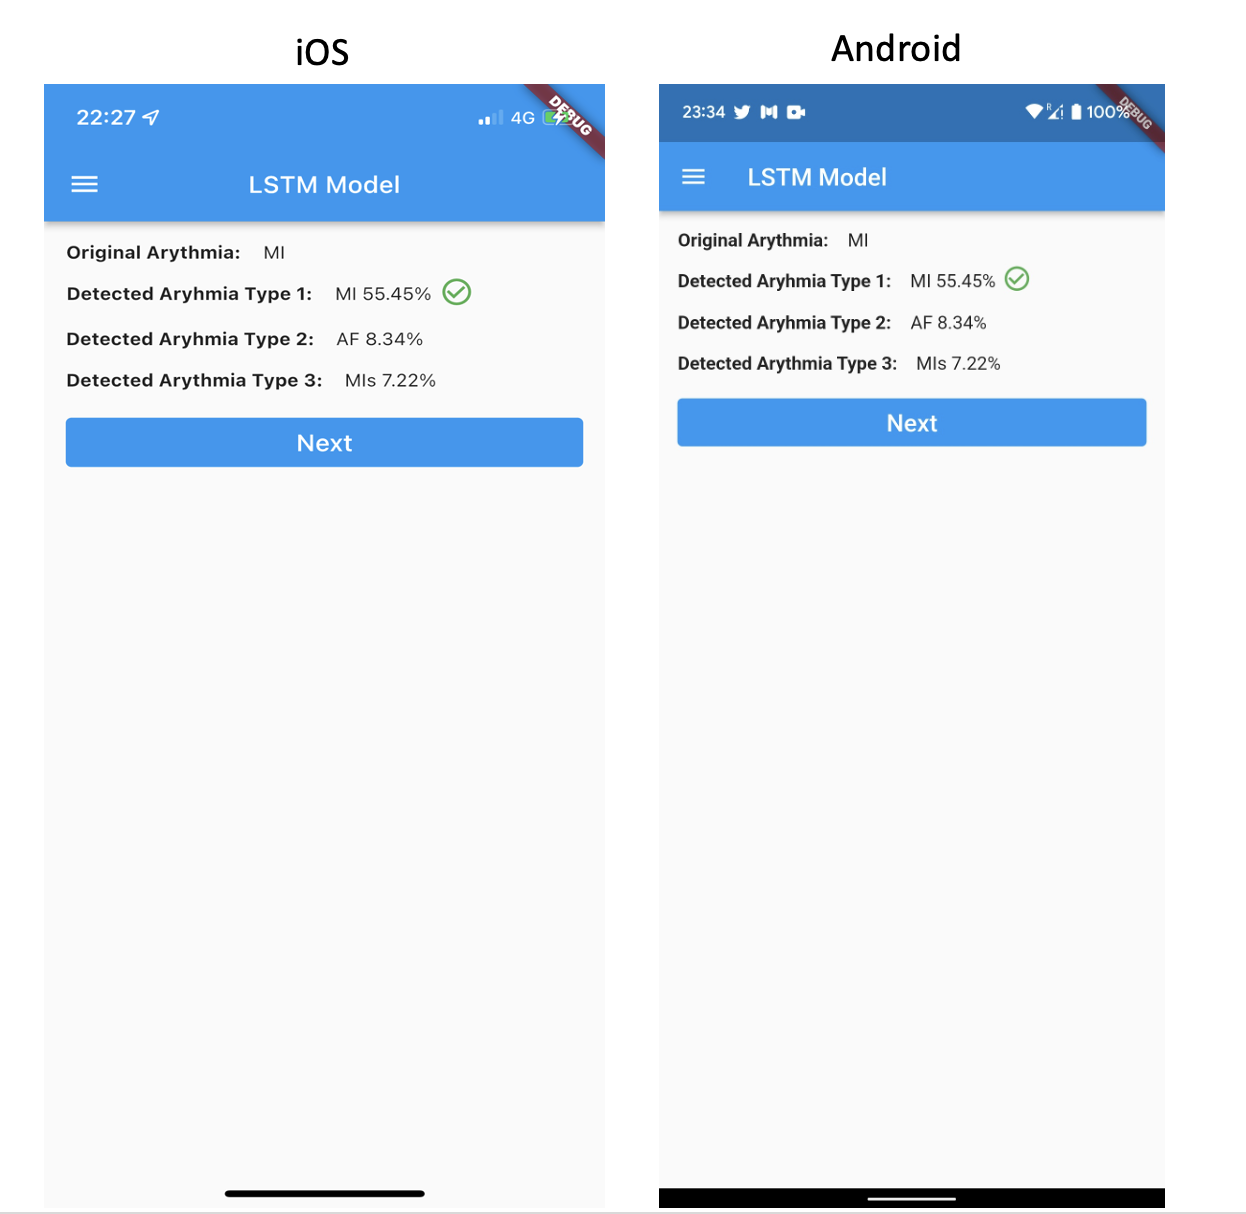
\includegraphics[scale=0.4]{img/lstm_deployment.png}
\caption{iOS and Android LSTM model classification example}
\label{dnn_deloyment}
\end{figure}

\textbf{Team \# 2}

For team \# 2, as they were using end to end model to classify 12-lead ECG, so for each input after pre processing was saved as one csv file instead .mat file in original dataset and age, sex and dx is saved separately as well in other csv file to provide it to the model. As team \# 2 was using ensemble model, combining 5 of them to output the results for final classification there has been post processing done on mobile application as it was in original source code provided by \ref{fig:team_two_network_2}. If we look at closely their model is doing multi class classification instead of predicting one arythmia at time because a patient can have more than one arythmia. Also, during prediction probabilities are divided into for how many arythmias its predict. For example if the model is predicting two different arythmia based on 12-lead ECG it will make whole precentage as 200\% instead of 100\%. 

\begin{figure}[H]
\centering
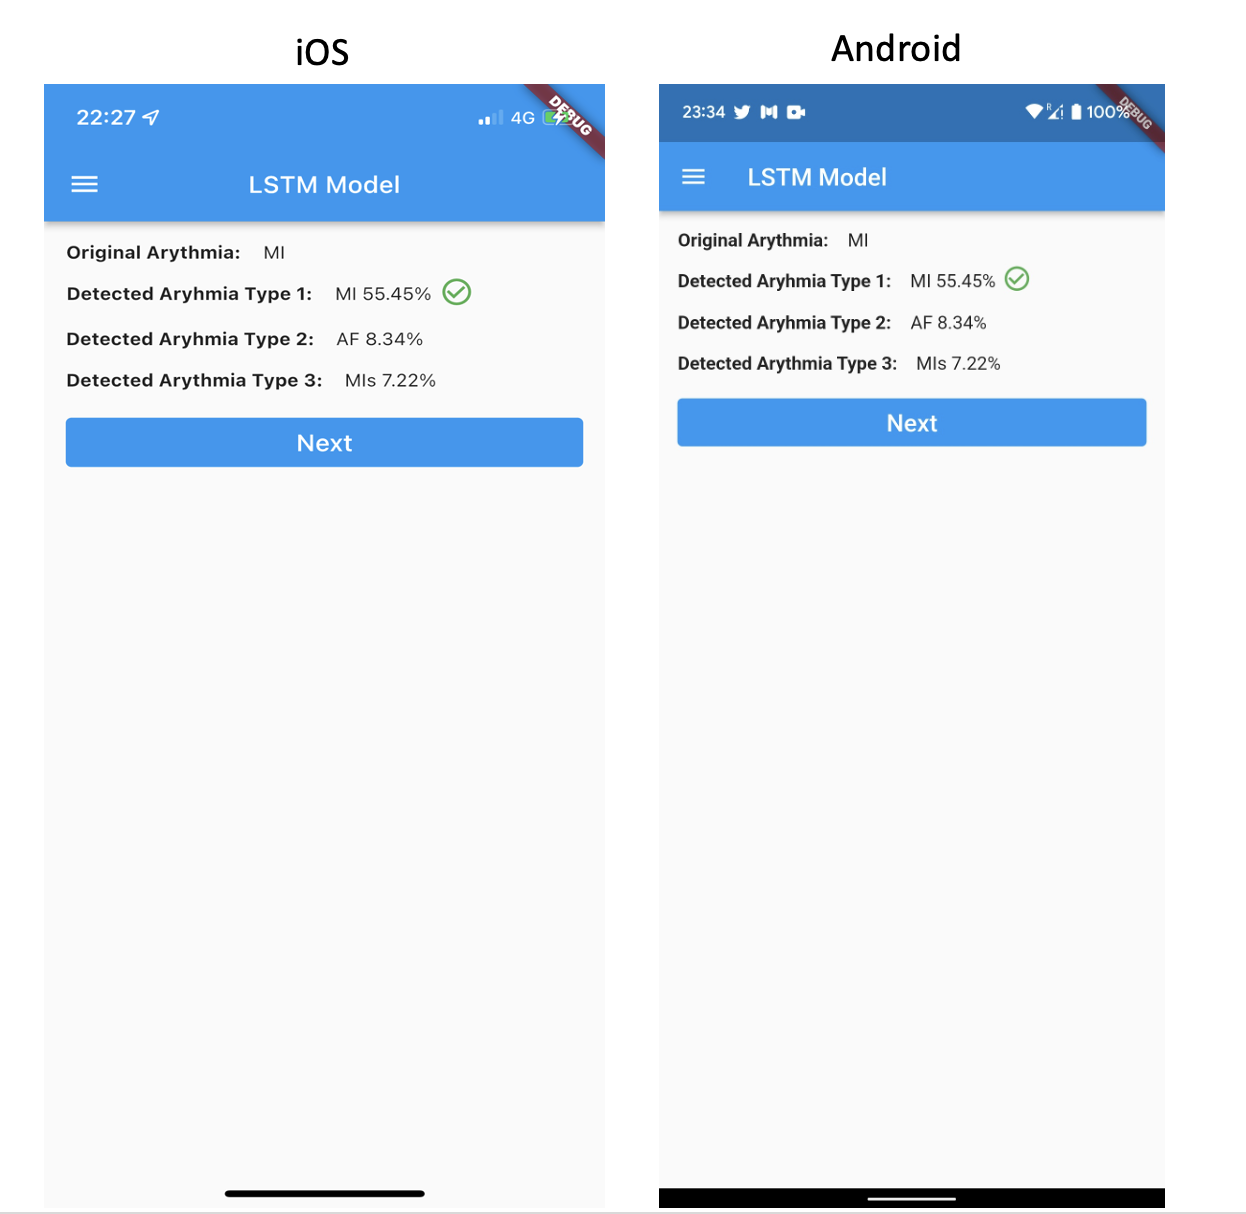
\includegraphics[scale=0.4]{img/lstm_deployment.png}
\caption{iOS and Android Team \# 2 model classification example}
\label{dnn_deloyment}
\end{figure}




\section{Federated Learning} \label{5FL}

Leveraged on the Centralized Learning method mentioned, it is time to immerse in the Federated Learning (FL) approach executed for this ECG dataset. With the CL it was possible to get an overall performance with the best techniques and scenarios to be applied. To deal with the FL proposed, there were two possible ways to work with the database in a Federated context. Those possibilities will be explained in the following chapters.

\subsection{IID approach}

This approach was based on the idea of using the whole dataset containing 41,894 registers and divide it in 4 different datasets (local nodes). As a parenthesis, the decision of the number of local nodes was based on selecting at least 30 diagnoses for the rarest arrhythmia. Due to the stratified random splitting, the mentioned data in each local node (or client) will be Independent and Identically Distributed (IID) \ref{proposed_approaches}. This scenario is not completely realistic since usually the ECGs shared in multiple devices are Non-IID. Nevertheless, it is worth to try and see how the FL approach will perform over the data.

\begin{figure}[H]
\centering
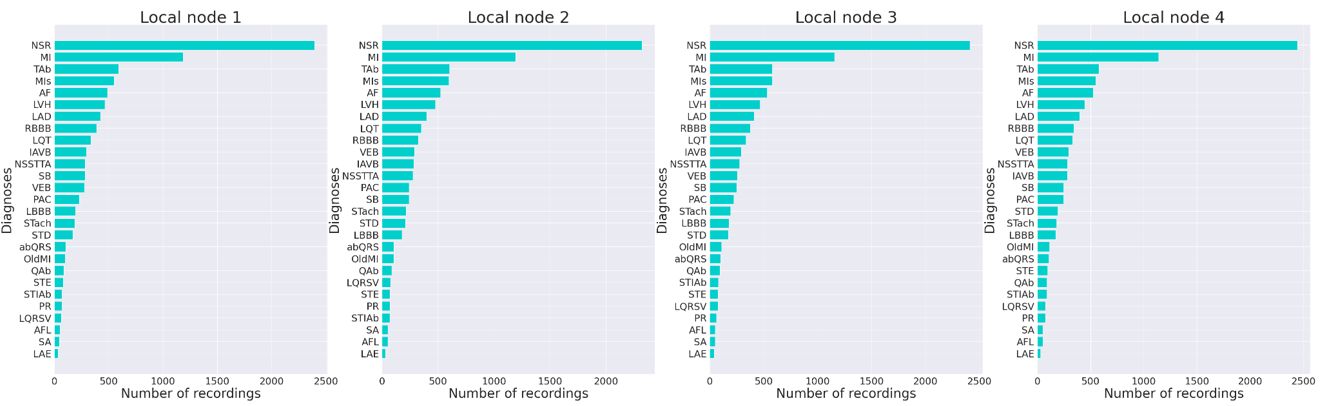
\includegraphics[scale=0.4]{img/fl_label_distro_filtered.png}
\caption{Label distribution for the filtered dataset by each local node}
\label{fig:fl_label_distro_filtered}
\end{figure}

As depicted in figure \ref{fig:fl_label_distro_filtered}, the distribution among the 4 local nodes seems IID. The later means that the diagnoses along the devices will be the same. Besides, each local node contains 9,426 recordings. The same occurs for the ROS and SMOTE datasets when dividing them in 4 clients, as is shown inf figures \ref{fig:fl_label_distro_filtered_ROS_SMT}. Of course, in this case all the diagnoses have almost the same participation across the nodes, making them IID and balanced.

\begin{figure}[H]
\centering
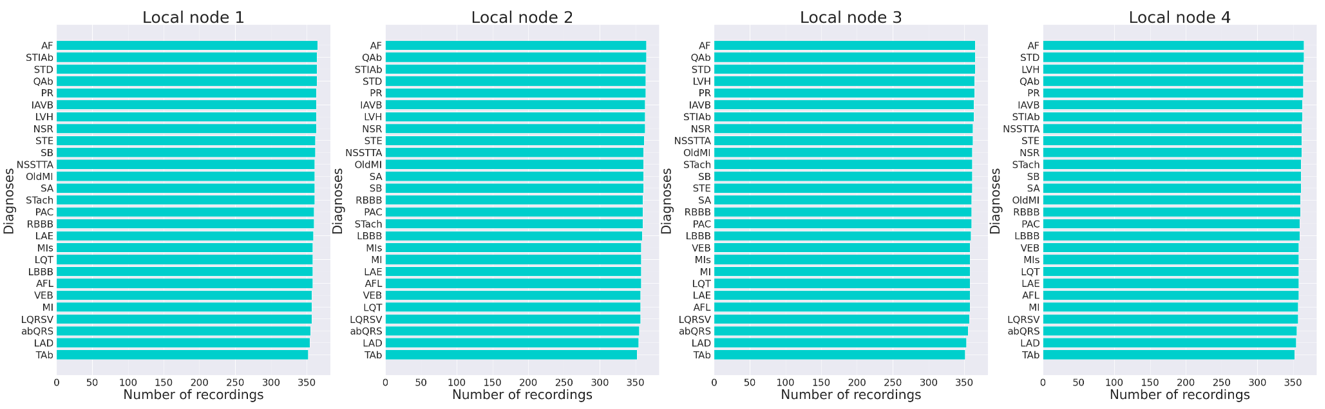
\includegraphics[scale=0.4]{img/fl_label_distro_filtered_ROS_SMT.png}
\caption{Label distribution for the ROS and SMOTE datasets by each local node}
\label{fig:fl_label_distro_filtered_ROS_SMT}
\end{figure}

Once the four datasets were settled, the modelling part can be performed. As a reminder, in the FL technique, each local node will train a model and later it will send the weights to a global node where the weights are averaged and updated back in each client. Then, the DNN and LSTM methodologies were used to classify the ECG's arrhythmias. It is relevant to highlight that Catboost and XG-Boost were not employed in this step. The former was discarded for its low performance and the latter due to its huge training time. Moreover, it the consulted bibliography, it is not common to use those ML techniques within the FL.

\begin{figure}[H]
\centering
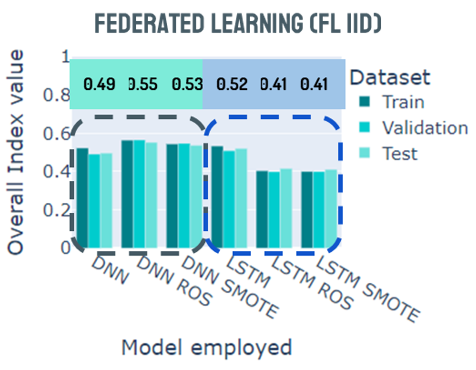
\includegraphics[scale=0.6]{img/fl_iid_methods.png}
\caption{Overall Index for methods employed in Federated Learning (FL)}
\label{fig:fl_iid_methods}
\end{figure}

As depicted in figure \ref{fig:fl_iid_methods}, the best results where obtained using the DNN with the ROS datasets. The later got an overall index of 0.55 in the test set. On the other hand, the best performance for LSTM was obtained with the original data, although it is worst than the DNN ROS model. The latter means that applying oversampling techniques doesn't improve the result of the models in the LSTM approach. But, when using ROS, the performance of the FL model is the most useful compared to all the techniques.

\begin{figure}[H]
\centering
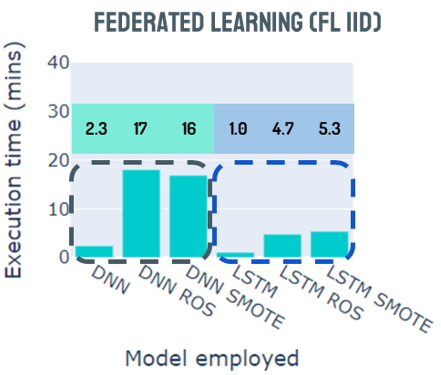
\includegraphics[scale=0.6]{img/times_fl_iid.png}
\caption{Execution times for the methods used in FL IID approach}
\label{fig:times_fl_iid}
\end{figure}

Analyzing figure \ref{fig:times_fl_iid} it is possible to get that the oversampling techniques cause the running time to increase \cite{fl28}. In detail, the slowest approach ended up being the DNN ROS with 17 minutes. Comparing the results to the CL approach, the DNN method with FL runs faster with similar results. On the other hand, DNN ROS and SMOTE ran slower and with a slower performance than the CL. Finally, LSTM, in general, has a lower performance than DNN, but runs faster.

With FL it is possible to control the performance that the models has in each local node. The latter is relevant to understand if there is some node that is under-performing, compared to the others.

\begin{figure}[H]
\centering
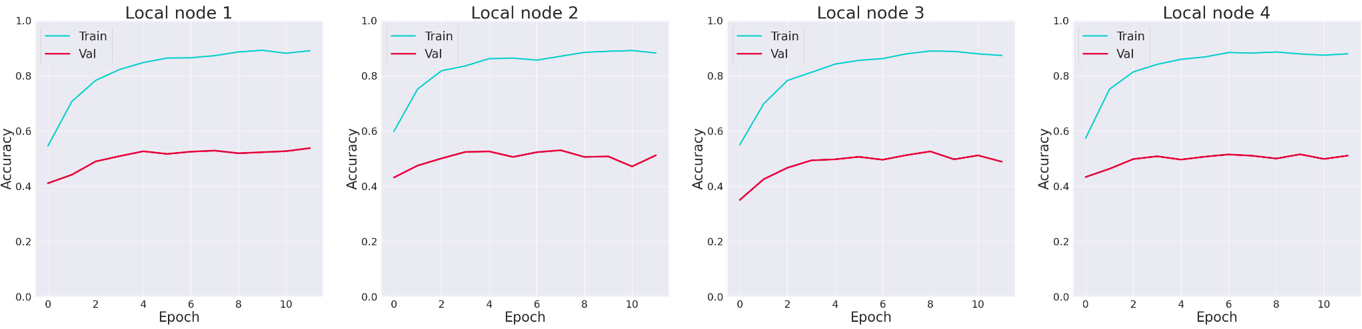
\includegraphics[scale=0.4]{img/iid_local_nodes_acc.png}
\caption{Train and Validation accuracy among local nodes for DNN ROS}
\label{fig:iid_local_nodes_acc}
\end{figure}

In figure \ref{fig:iid_local_nodes_acc} is depicted the behaviour of each local node with respect to the accuracy for both the training and validation datasets. In general, the models among the clients have a similar behaviour. All of them get stabilized around the 5th epoch. It is important to clarify that the accuracy for train and validation seems considerably far from each other. The latter would mean that the models are overfitting. Nevertheless, the train sample is an oversampled data while the validation is a part of the original data, then, it is expected to such a behaviour.

In a a FL environment there is a concept called \textbf{communication round} (comm round). The latter begins when a model is trained inside each one of the local nodes. Later the weights of the models are passed to the global node to be aggregated there. And finally, the communication round finishes when each local model is updated with the new weights. Then, it is expected that in each comm round the performance of the model increases. Moreover, it should get stable after some trials.

\begin{figure}[H]
\centering
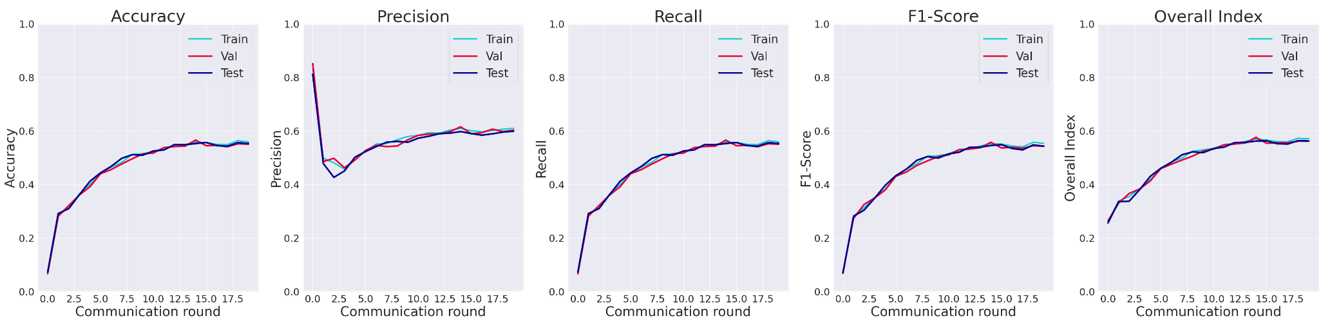
\includegraphics[scale=0.4]{img/comm_round_metrics_DNNROS.png}
\caption{Metrics along communication rounds for DNN ROS (the best model)}
\label{fig:comm_round_metrics_DNNROS}
\end{figure}

Figure \ref{fig:comm_round_metrics_DNNROS} establishes the behaviour of each metrics along the communication rounds. As expected, the performances gets stable after the 15th comm round approximately. It is relevant to notice that in the first comm round the Precision starts high and the Recall low. But after some updates both measures get steady. Moreover, the curves for train, validation and test are close. The latter means that there are not signals of overfitting.


\begin{figure}[H]
\centering
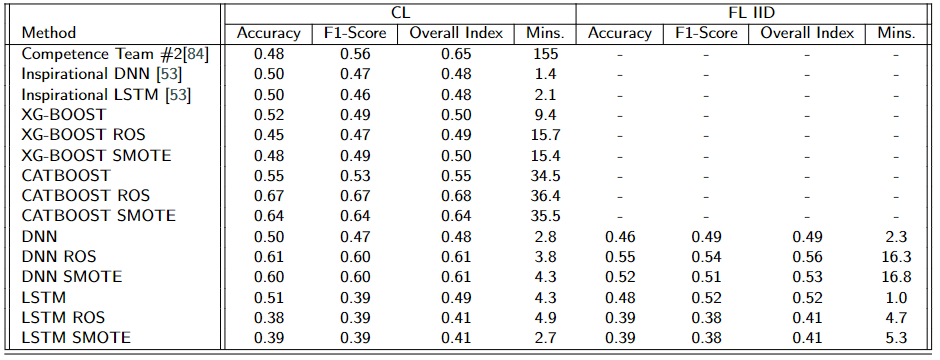
\includegraphics[scale=0.55]{img/metrics_CL_FLIID.png}
\caption{Metrics for Centralized (CL) and IID Federated Learning (FL -IID) in the test data set. Also included execution time for  training in minutes (Mins.)}
\label{figure:metrics_CL_FLIID}
\end{figure}

The table \ref{figure:metrics_CL_FLIID} includes a summary of all the techniques implemented with the data in the IID and Centralized (CL) approaches. It is remarkable to mention that Catboost and DNN ROS outperformed the model implemented by the second team of the competence.

\subsection{Non-IID approach}

This method was based on the idea of taking four random samples with repetition from the entire dataset of 41,894 registrations (local nodes). The given data in each local node (or client) will be Non-IID \ref{proposed_approaches} approaches because to the unstratified random sampling. Because most ECGs shared across several devices are Non-IID, this scenario is far more plausible.

\begin{figure}[H]
\centering
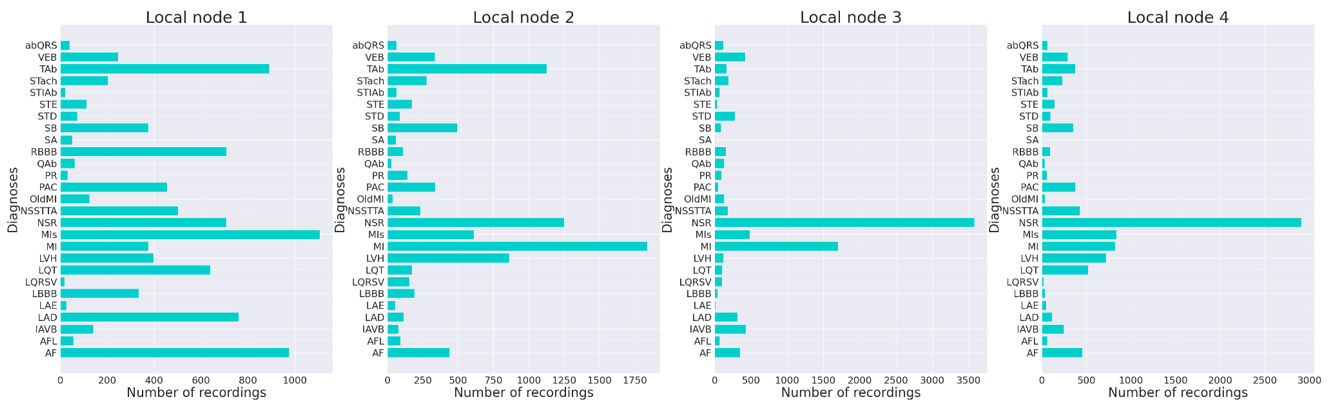
\includegraphics[scale=0.4]{img/fl_label_distro_filtered_noniid.png}
\caption{Label distribution for the filtered dataset by each local node for the Non-IID case}
\label{fig:fl_label_distro_filtered_noniid}
\end{figure}

The distribution among the four local nodes appears Non-IID, as shown in figure \ref{fig:fl_label_distro_filtered_noniid}. The latter implies that diagnosis along the devices will differ. Furthermore, each local node has around 9,426 records. The ROS and SMOTE datasets behave similarly when divided into four clients, as demonstrated in figure \ref{fig:fl_label_distro_filtered_ROS_SMT} Naturally, all of the diagnoses in this scenario have nearly equal participation throughout the nodes, making them IID and balanced.

The modeling was done again when the four datasets were extracted. The ECG's arrhythmias were then classified using the DNN and LSTM techniques. Catboost and XG-Boost were not used in this scenario for the same reasons as previously stated.

\begin{figure}[H]
\centering
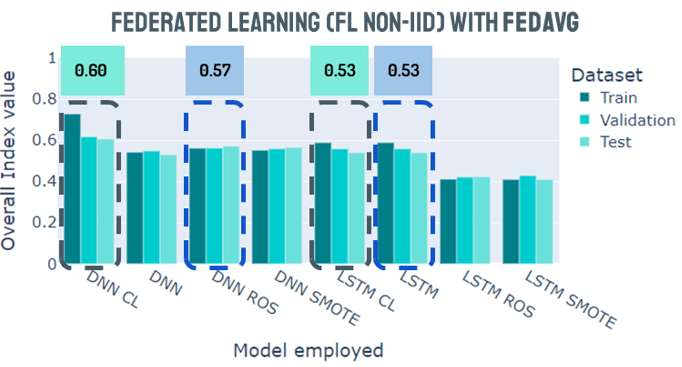
\includegraphics[scale=0.6]{img/fl_noniid_methods.png}
\caption{Overall Index for methods employed in Federated Learning (FL) Non-IID case}
\label{fig:fl_noniid_methods}
\end{figure}

A centralized learning strategy (CL) was used in this scenario. The prior method implied appending the four created local nodes and utilizing that data to train a model (for both DNN and LSTM). Then, it is intended that the other algorithms will be as near to the CL approach as possible. The best results were obtained using the DNN with the ROS datasets, as shown in figure \ref{fig:fl_noniid_methods}, while the DNN and DNN LSTM techniques also performed well in this scenario. In the test set, the former received an overall index of 0.57. The highest performance for LSTM, on the other hand, was obtained with the original data (LSTM), however it was worse than the DNN ROS model. This suggests that using oversampling approaches does not improve the results of the models in the LSTM approach in this circumstance. However, when using ROS, the FL model's performance is the most useful of all the strategies.

\begin{figure}[H]
\centering
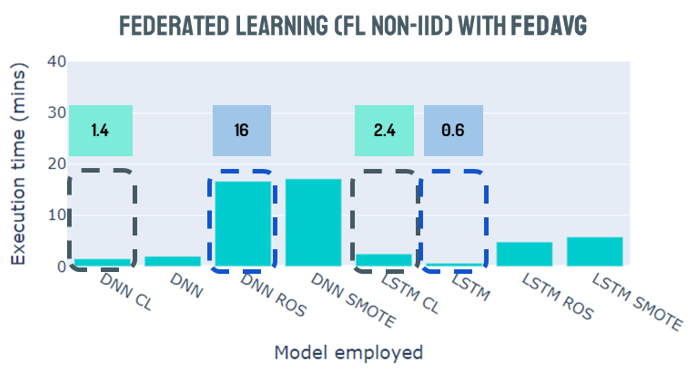
\includegraphics[scale=0.6]{img/times_fl_noniid.png}
\caption{Execution times for the methods used in FL Non-IID approach}
\label{fig:times_fl_noniid}
\end{figure}

It is possible to obtain the running times for the algorithms by analyzing picture \ref{fig:times_fl_noniid}. The DNN ROS method was the slowest, clocking in at 16 minutes. When compared to the CL method, the DNN method with FL is faster and produces equivalent results. The same thing happens with DNN ROS and SMOTE. Finally, while LSTM has lesser performance than DNN in general, it is significantly faster.

As mentioned in \ref{non_iid_handling}, there are some methods used to handle the Non-IID condition that may affect the performance of the models in a FL architecture. Therefore, in this work I applied the \textbf{FedProx} aggregation technique to evaluate if the performance of the models can be better. 

\begin{figure}[H]
\centering
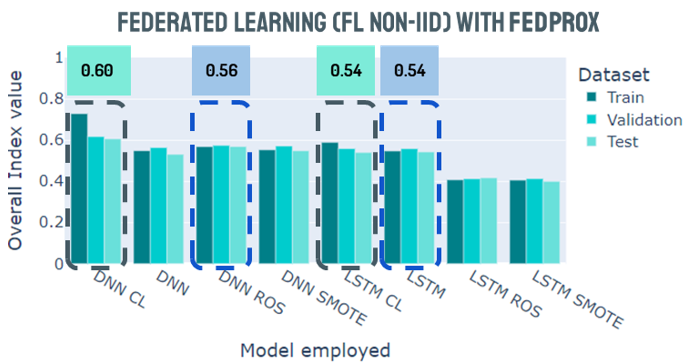
\includegraphics[scale=0.6]{img/fl_noniid_methods_fedprox.png}
\caption{Overall Index for methods employed in Federated Learning (FL) Non-IID case with FedProx}
\label{fig:fl_noniid_methods_fedprox}
\end{figure}

As depicted in figure \ref{fig:fl_noniid_methods_fedprox}, using FedProx aggregation didn't make an improvement in the classification power of the models. Nevertheless, when looking at figure \ref{fig:times_fl_noniid_fedprox} the times spent to train the algorithms, the DNN ROS reduced in approximately 25\% the execution time.  That's an advantage of FedProx since it is important to have models that can train faster in the devices (hospitals).

\begin{figure}[H]
\centering
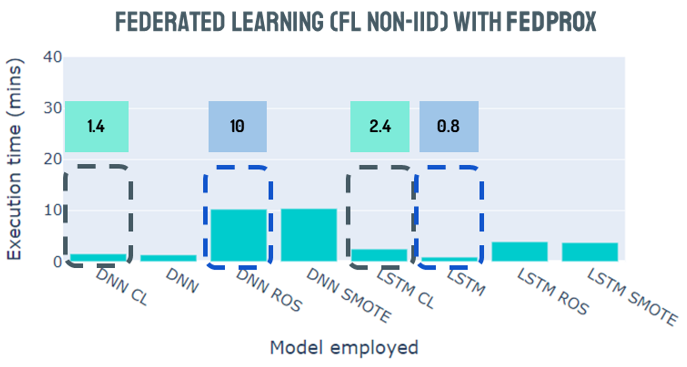
\includegraphics[scale=0.6]{img/times_fl_noniid_fedprox.png}
\caption{Execution times for the methods used in FL Non-IID approach with FedProx}
\label{fig:times_fl_noniid_fedprox}
\end{figure}

Along with the experimentation we wanted to check the behaviour of the models when the number of local nodes was different to 4. Then, we simulated scenarios by changing the number of clients from 2 to 10. In each execution we had to train a centralized model (CL) to see how well the FL training was fitting regarding that CL reference point.

\begin{figure}[H]
\centering
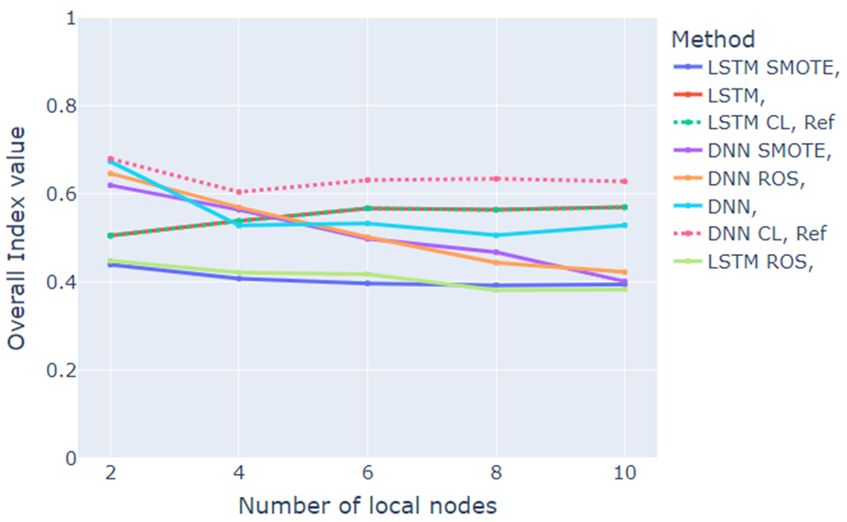
\includegraphics[scale=0.6]{img/change_local_nodes_metrics_fedavg.png}
\caption{Overall index changing number of local nodes with FedAvg}
\label{fig:change_local_nodes_metrics_fedavg}
\end{figure}

Figure \ref{fig:change_local_nodes_metrics_fedavg} represents the Overall Index measured in the test dataset for all the methods used by changing the number of local nodes. DNN CL and LSTM CL are the references model trained with all the data appended in on single dataset (centralized or common learning). Then, we can see that when considering four or less local nodes the best solution is DNN ROS since it is close enough to the reference model. On the other hand, when using more than 4 local nodes best solution is LSTM, keeping more or less constant when increasing the number of clients.

\begin{figure}[H]
\centering
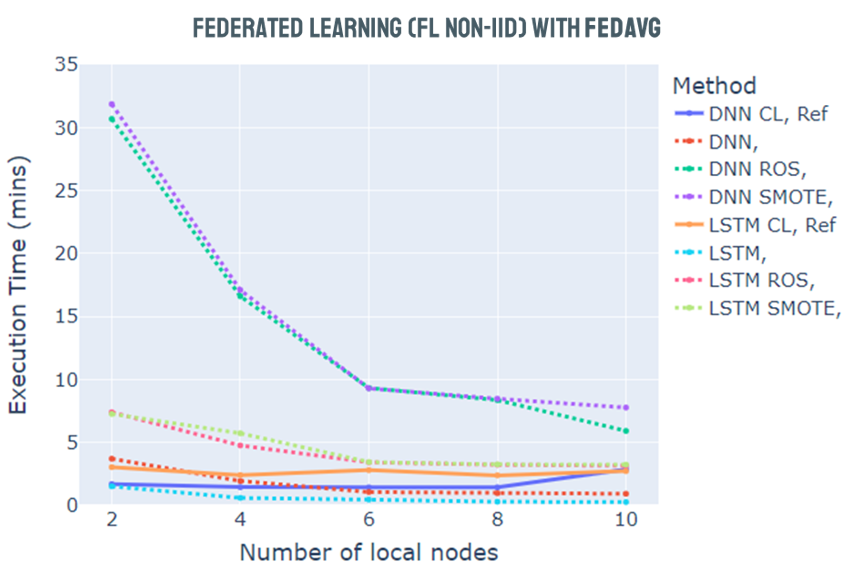
\includegraphics[scale=0.6]{img/change_local_nodes_time_fedavg.png}
\caption{Running time changing number of local nodes with FedAvg}
\label{fig:change_local_nodes_time_fedavg}
\end{figure}


Comparing the running time while changing the number of local nodes is demonstrated in figure \ref{fig:change_local_nodes_time_fedavg}. In general, the higher the number of local nodes, the faster the algorithms run. Moreover, DNN ROS and SMOTE drastically decreased the running time by increasing the local nodes. Nevertheless, the performance also decreased. In the case of LSTM, it had the highest performance with the fastest running time when increasing the number of clients.

\begin{figure}[H]
\centering
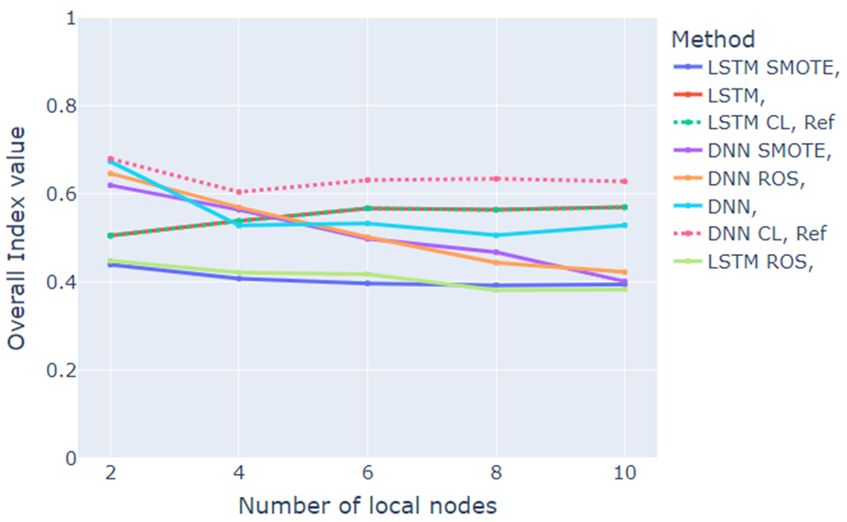
\includegraphics[scale=0.6]{img/change_local_nodes_metrics_fedavg.png}
\caption{Overall index changing number of local nodes with FedProx}
\label{fig:change_local_nodes_metrics_fedprox}
\end{figure}

Figure \ref{fig:change_local_nodes_metrics_fedprox} represents the Overall Index measured in the test dataset for all the methods used by changing the number of local nodes using a FedProx aggregation method. We can see that the behaviour of the models doesn't show a significant change when utilizing FedProx. On the contrary, using the mentioned aggregation generated an improvement over the performance of  DNN, DNN ROS and DNN SMOTE methodologies as depicted in \ref{fig:change_local_nodes_time_fedprox}.

\begin{figure}[H]
\centering
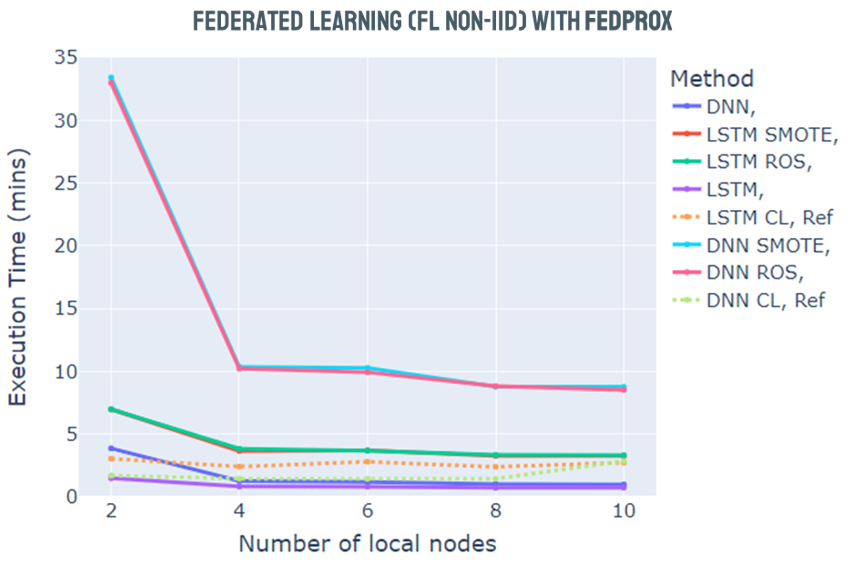
\includegraphics[scale=0.6]{img/change_local_nodes_time_fedprox.png}
\caption{Running time changing number of local nodes with FedProx}
\label{fig:change_local_nodes_time_fedprox}
\end{figure}